\documentclass{article}
% Useful packages
\usepackage{amsmath} % Required for advanced math typesetting
\usepackage{graphicx} % Required for inserting images
\usepackage{xcolor} % Required for color definitions
\usepackage{listings}
\usepackage{tcolorbox} % Required for creating boxes
\usepackage{float} % Required for controlling the position of images
\usepackage{hyperref} % Required for URLs and hyperlinks


% Code settings
\lstset{
    language=C,
    basicstyle=\ttfamily\small,
    keywordstyle=\color{blue},
    commentstyle=\color{green!50!black},
    stringstyle=\color{orange},
    showstringspaces=false,
    breaklines=true,
    frame=single,
    numbers=left,
    numberstyle=\tiny,
    stepnumber=1
}

\setlength{\parindent}{0pt}

\title{SEAI\_2024\_R12}
\author{Giulio Capecchi, Jacopo Niccolai}
\date{December 2024}


\begin{document}

\maketitle

\vspace{3cm}
\begin{figure}[H]
    \centering
    
\includegraphics[width=0.6\textwidth]{assets/unipi.png}
    \label{fig:unipi_logo}
\end{figure}

\newpage

\tableofcontents

\newpage

\section{Introduction}
This project focuses on the synthesis of the forward pass for two types of neural network architectures: a \textbf{Multilayer Perceptron (MLP)} and a \textbf{Convolutional Neural Network (ConvNet)}, implemented on an FPGA (Field Programmable Gate Array).  To achieve this, the network parameters were first obtained using Python and the \textit{PyTorch} library; these were subsequently hardcoded into \texttt{C} code, enabling the hardware synthesis process.


\begin{figure}[H]
    \centering
    
\includegraphics[width=0.5\textwidth]{assets/vitis-hls.png}
    \caption{Xilinx Vitis HLS}
    \label{fig:vitis_hls}
\end{figure}

\textbf{Vitis Unified Software Platform} is a comprehensive suite designed to accelerate the development of applications on FPGAs, Adaptive SoCs, and ACAPs (Adaptive Compute Acceleration Platforms). By combining high-level software programming techniques with hardware-optimized implementations, Vitis enables developers to write applications in \textit{C}, \textit{C++}, or \textit{OpenCL} while leveraging hardware-specific optimizations for enhanced performance. In this project, Vitis was used to synthesize neural network architectures - MLP and ConvNet - onto an FPGA. Its \textbf{High-Level Synthesis (HLS)} tools allow for rapid prototyping and optimization of the \textit{C} code, ensuring efficient resource utilization, parallelism and low-latency execution. The platform's ability to integrate high-level design, simulation, and hardware synthesis simplifies the workflow, bridging the gap between software and hardware development.


\section{Project Description}
\subsection{Workflow Overview}
The project follows a structured workflow. For each neural network architecture, a Jupyter Notebook is provided in the \texttt{PyTorch} folder. As the name of the folder suggests, these were constructed and trained using the \textit{PyTorch} library. Once trained, the weights and biases were exported to be hardcoded into the corresponding \texttt{C} implementation. The \texttt{C} code was designed to be compatible with FPGA synthesis tools, such as Vitis HLS/Vivado, and can be found inside the \texttt{HLS-Implementation} folder.

\subsection{Jupyter Notebooks}
For each network architecture, a Jupyter Notebook was created to train the model and export the parameters. These notebooks are similar to each other since they contain almost the same steps for each neural network. Their main sections are:
\begin{itemize}
    \item \textbf{Dataset Preparation}: Loading the chosen dataset to train the model.
    \item \textbf{Model Definition}: Defining the neural network architecture.
    \item \textbf{Model Training}: Training the model on the dataset, ensuring that it converges to a satisfactory accuracy.
    \item \textbf{Exporting Parameters}: Extracting the weights and biases for the forward pass to a text file.
\end{itemize}

\begin{figure}[H]
    \centering
    
\includegraphics[width=0.3\textwidth]{./assets/jupyter-notebooks.png}
    \caption{Jupyter Notebooks logo}
    \label{fig:jupyter-notebooks}
\end{figure}



\subsection{C Implementation}
As for the Jupyter Notebooks, the \texttt{C} code is structured in a similar way for each architecture. There are always \textit{three files} provided:
\begin{itemize}
    \item \texttt{architecture.c}: contains the forward pass function and the definition of the architecture.
    \item \texttt{architecture.h}: contains the definition of the architecture and the prototype of the forward pass function.
    \item \texttt{testbench.c}: reads the dataset and contains the main function to test the forward pass function.
\end{itemize}

To optimize the C implementation for hardware synthesis, specific \textbf{HLS directives} were applied to critical portions of the code. These directives guide the High-Level Synthesis (HLS) tool to produce more efficient hardware designs by controlling resource allocation, loop unrolling, and pipeline creation. The two main directives used in this project are:

\begin{itemize}
    \item \textbf{\texttt{HLS INLINE}}: This directive forces the complete insertion of the body of a function or loop directly at the point where it is called, eliminating the overhead associated with function calls or separate hardware resource allocation. By doing so, it reduces latency by eliminating function call delays. However, it may increase the usage of the hardware area, as the logic is replicated wherever the function is called. It is typically used for simple or frequently invoked functions to reduce latency.
    
    \item \textbf{\texttt{HLS PIPELINE}}: This directive breaks a loop or function into multiple stages (pipeline), allowing multiple iterations or operations to execute simultaneously, thereby increasing the design's throughput. It enables the processing of new iterations in every clock cycle (or at specific intervals called \textit{ initiation interval (II)}). The options for this directive include \texttt{II=N} (to specify the interval between iterations, such as 1 clock cycle) and \texttt{rewind} (to automatically restart the loop after completion). It is typically used in loops that process large amounts of data to maximize throughput in repetitive operations.

\end{itemize}

It is important to note that the directives discussed in this section represent only a subset of the directives executed by the HLS compiler during the synthesis process. These directives were explicitly added to address specific warnings and improve the design's performance. They were placed on the exact lines of code where they were required to resolve issues or optimize critical sections of the implementation.


\paragraph{Hardcoding Network Parameters}
The network's weights and biases, extracted from the trained PyTorch model, were directly integrated into the \textit{C} implementation as hardcoded values. This allows the FPGA hardware to access the pre-trained parameters directly during the forward pass, avoiding external memory accesses. The process of exporting these parameters is detailed in \ref{sec:exporting-parameters}. After extraction, the parameters were organized in the \texttt{C} code as arrays within dedicated data structures. These structures and their integration will be explained in detail later on for each architecture.

\subsection{Loading the project into the Vitis Unified IDE}
The project was loaded into the Vitis Unified IDE to synthesize the \texttt{C} code and generate the corresponding hardware description. The IDE provides a comprehensive environment for developing, debugging, and deploying applications on Xilinx devices. The following steps has to be followed to load the project into the Vitis Unified IDE:
\begin{enumerate}
    \item Open the Vitis Unified IDE and under \texttt{HLS Development} select \texttt{Create component...}.
    \item Click on \texttt{Create Empty HLS Component}. A new window should appear, where you can specify the component name and location.
    \item You will then be asked about the configuration file : you can either provide one or click on \textit{next} and let the IDE create one for you.
    \item In the following page, specify in the \texttt{Top Function} field the name of the function that you want to synthesize: this should be the one that you want to test on the FPGA. In our case, it is the forward pass function (the name is \texttt{forward} for all the networks we worked on).
    \item  Click on next and select a device: it should have enough resources to contain the design.
    \item Click on \texttt{next} until you reach the \texttt{finish} button. Click on it to create the project.
\end{enumerate}

\begin{figure}[H]
    \begin{minipage}{0.4\textwidth}
        \raggedright
        Once done, you should see on the left a structure similar to the one provided in the image. Inside \texttt{Settings} you can find the configuration file for the project, but the simpler way to add the necessary files to the project is to right-click on \texttt{Sources} and then add the \texttt{C} and {header} files. Do the same for the \texttt{testbench}, where you should add the \texttt{txt} file containing the dataset and the \texttt{testbench.c} file, specific for the current component.
        \\To "run" the project, you can then use the buttons on the bottom of this section (\texttt{Run, C Synthesis, C/RTL Cosimulation, Package, Implemenattion}). Their usage will be explained later on.
    \end{minipage}
    \hfill
    \begin{minipage}{0.4\textwidth}
        \centering
        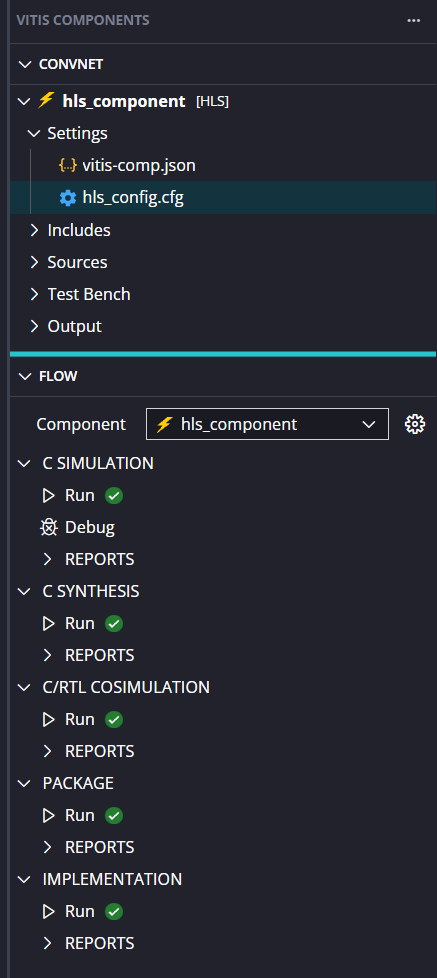
\includegraphics[width=\textwidth]{assets/IDE-structure.png}
        \caption{IDE Structure}
        \label{fig:ide_structure}
    \end{minipage}
\end{figure}


\section{Multi-Layer Perceptron (MLP)}
Let's analyze the implementation of the forward pass for a Multi-Layer Perceptron. The forward pass for an MLP consists of propagating the input through a series of layers, each followed by an activation function.
The code for it can be found inside the \texttt{PyTorch} folder, that contains the notebooks used to train the models and export their parameters.

\subsection{Dataset}
The MLP was trained using the well-known \textit{Iris} dataset, which contains 150 samples of iris flowers, each with four features and a class label (the last value of each row).
There is a total of three classes: \textit{setosa}, \textit{versicolor}, and \textit{virginica}.
The dataset was split into training and test sets, with 80\% of the samples used for training and 20\% for testing.
\\\\An example of the dataset is shown below:

\begin{tcolorbox}[colback=gray!5, colframe=black, rounded corners, boxrule=0.1mm]
\textbf{\textcolor{blue}{sepal\_length,sepal\_width,petal\_length,petal\_width,species}} \\
5.1,3.5,1.4,0.2,setosa \\
5.7,2.8,4.5,1.3,versicolor \\
6.1,2.6,5.6,1.4,virginica \\
...
\end{tcolorbox}

The dataset's labels were encoded as integers using the Scikit-learn \texttt{LabelEncoder} class, which maps each class to a unique integer value. To facilitate its further usage inside the \texttt{C} implementation, this encoded version of the dataset was saved to a txt file, \textit{iris\_dataset\_encoded.txt}.

\subsection{PyTorch Model}
\subsubsection{Model Architecture}
The architecture of the MLP model consists of three fully connected layers.  
The input layer has 4 neurons, corresponding to the 4 features of the Iris dataset. 
The first and second hidden layers each have 10 neurons, while the output layer has 3 neurons, corresponding to the 3 classes of the Iris dataset.  
The ReLU activation function is applied after each dense layer, except for the output layer.  
\\\\The ReLU function is defined as:  
\begin{center}
$\operatorname{ReLU}(x) = \max(0, x)$
\end{center}

The forward pass of the model applies the ReLU activation function after the first and second layers.  
\\\\\\The model was implemented using the \textit{PyTorch} library as follows, by defining a custom class \texttt{MLP} that inherits from \texttt{nn.Module}:

\begin{lstlisting}[language=Python]
# Define the MLP model
class MLP(nn.Module):
    def __init__(self):
        super(MLP, self).__init__()
        self.fc1 = nn.Linear(4, 10)
        self.fc2 = nn.Linear(10, 10)
        self.fc3 = nn.Linear(10, 3)
    
    def forward(self, x):
        x = torch.relu(self.fc1(x))  # Apply ReLU after first layer
        x = torch.relu(self.fc2(x))  # Apply ReLU after second layer
        x = self.fc3(x)  # Output layer (no activation)
        return x
\end{lstlisting}


\subsubsection{Model Training}
For the training phase, we first defined the model, loss function, and optimizer.
We utilized the \textit{CrossEntropyLoss} loss function, which is commonly used for multi-class classification problems, and the \textit{Adam} optimizer, which is an adaptive learning rate optimization algorithm.

\begin{lstlisting}[language=Python]
model = MLP()

# Check if GPU is available
device = torch.device('cuda' if torch.cuda.is_available() else 'cpu')
model = model.to(device)

criterion = nn.CrossEntropyLoss()
optimizer = optim.Adam(model.parameters(), lr=0.01)
\end{lstlisting}

The following code snippet demonstrates the trainign process using \textit{PyTorch}. The model is trained for 100 epochs.

\begin{lstlisting}[language=Python]
# Training loop
NUM_EPOCHS = 100
for epoch in range(NUM_EPOCHS):
    model.train()
    running_loss = 0.0
    for inputs, labels in train_loader:
        inputs, labels = inputs.to(device), labels.to(device)
        
        optimizer.zero_grad()
        outputs = model(inputs)
        loss = criterion(outputs, labels)
        loss.backward()
        optimizer.step()

        running_loss += loss.item()

    # Evaluate the model after each epoch
    model.eval()
    correct = 0
    total = 0
    with torch.no_grad():
        for inputs, labels in test_loader:
            inputs, labels = inputs.to(device), labels.to(device)
            outputs = model(inputs)
            _, predicted = torch.max(outputs.data, 1) # Get the class index with the highest probability
            total += labels.size(0)
            correct += (predicted == labels).sum().item()

    accuracy = correct / total

    if (epoch + 1) % 10 == 0:
        print(f'Epoch [{epoch+1}/{NUM_EPOCHS}], Loss: {running_loss/len(train_loader):.4f}, Accuracy: {accuracy * 100:.2f}%')
\end{lstlisting}

The results of the training process are reported in the table below:
\begin{table}[H]
    \centering
    \begin{tabular}{|c|c|c|c|}
        \hline
        \textbf{Epoch} & \textbf{Loss} & \textbf{Train Accuracy} & \textbf{Test Accuracy} \\
        \hline
        10 & 0.3258 & 90.48\% & 88.89\% \\
        20 & 0.1060 & 97.14\% & 97.78\% \\
        30 & 0.1312 & 95.24\% & 97.78\% \\
        40 & 0.0853 & 97.14\% & 100.00\% \\
        50 & 0.0675 & 98.10\% & 100.00\% \\
        60 & 0.0971 & 96.19\% & 97.78\% \\
        70 & 0.0952 & 96.19\% & 97.78\% \\
        80 & 0.1020 & 96.19\% & 97.78\% \\
        90 & 0.0929 & 96.19\% & 97.78\% \\
        100 & 0.0788 & 94.29\% & 97.78\% \\
        \hline
    \end{tabular}
    \caption{\centering Training loss, train accuracy, and test accuracy of the MLP over 100 epochs.}
    \label{tab:mlp-training}
\end{table}


The training process shows that the model is able to achieve a high level of accuracy on both the training and test sets: this is to be expected given the simplicity of the Iris dataset and the effectiveness of the MLP architecture in solving such problems.
Given the relatively small dataset and the fact that the model achieves near-perfect accuracy on the test set, we can conclude that the model is generalizing well.

\subsubsection{Exporting Parameters}
\label{sec:exporting-parameters}
The trained model's parameters were exported to be hardcoded into the \texttt{C} implementation. The weights and biases of each layer were extracted and saved in a txt file, \textit{mlp\_weights.txt}, as shown below:
\begin{lstlisting}[language=Python]
import numpy as np

weights = {}
for name, param in model.named_parameters():
    weights[name] = param.detach().numpy()

# Print their shapes to verify the network architecture
for name, weight in weights.items():
    print(f"{name}: {weight.shape}")

import numpy as np

with open('./mlp_weights.txt', 'w') as f:
    for name, weight in weights.items():
        f.write(f"// {name}, shape: {weight.shape}\n")
        if weight.ndim == 2:  # Fully connected layer weights
            for row in weight:
                f.write("{" + ", ".join(map(str, row)) + "},\n")
        elif weight.ndim == 1:  # Biases or 1D weights
            f.write("{" + ", ".join(map(str, weight)) + "},\n")
\end{lstlisting}

\subsection{C Implementation}

The implementation for Vitis HLS of the MLP was produced with three files:
\begin{itemize}
    \item \texttt{mlp.c}, which contains the forward pass function, the activation function, and the definition of the MLP structure.
    \item \texttt{mlp.h}, which contains the definition of the MLP structure and the forward pass function prototype.
    \item \texttt{testbench.c}, which reads the \textit{iris\_dataset\_encoded.txt}  and contains the main function to test the forward pass function.
\end{itemize}
\subsubsection{MLP Structure}
\label{sec:mlp-structure}
The MLP structure was defined as follows (inside \texttt{mlp.h}):
\begin{lstlisting}
typedef struct {
    float weights[MAX_NEURONS][MAX_NEURONS]; // matrix
    float biases[MAX_NEURONS];   // biases of the layer
    float output[MAX_NEURONS];   // output of the layer
} Layer;

typedef struct {
    int num_layers;              // number of layers
    Layer layers[MAX_LAYERS];    // layers of the MLP (array of layers)
} MLP;
\end{lstlisting}

\texttt{MAX\_NEURONS} and \texttt{MAX\_LAYERS} are defined as 100 and 3, respectively.

\subsubsection{Forward Pass}
The forward pass for the MLP is implemented in \texttt{mlp.c} as a sequence of operations applied to each layer of the network. The function processes four input features through three layers, each defined by its respective weights and biases, to produce the predicted class index.
It is defined as follows:
\begin{lstlisting}
int forward(float input0, float input1, float input2, float input3) {
    const int input_sizes[4] = {4, 10, 10, 3}; 
    const int num_layers = 3;

    float current_input[MAX_NEURONS];
    float next_input[MAX_NEURONS];

    current_input[0] = input0;
    current_input[1] = input1;
    current_input[2] = input2;
    current_input[3] = input3;

    for (int i = 0; i < num_layers; i++) {
        #pragma HLS UNROLL
        Layer *layer = &mlp.layers[i];
        for (int j = 0; j < input_sizes[i + 1]; j++) {
            float sum = layer->biases[j];
            
            for (int k = 0; k < input_sizes[i]; k++) {
                sum += layer->weights[j][k] * current_input[k];
            }
            next_input[j] = reLu(sum);
        }

        for (int j = 0; j < input_sizes[i + 1]; j++) {
            current_input[j] = next_input[j];
        }
    }

    int max_index = 0;
    float max = current_input[0];
    for (int i = 1; i < NUM_CLASSES; i++) {
        #pragma HLS UNROLL
        if (current_input[i] > max) {
            max = current_input[i];
            max_index = i;
        }
    }
    return max_index;
}
\end{lstlisting}

As already explained, all weights and biases are hardcoded and directly integrated into the MLP definition at the top of \texttt{mlp.c}. These values are exported from the PyTorch model and were inserted manually into the code.
\\\\A notable feature of this implementation is the use of the \texttt{\#pragma HLS UNROLL} directive. This directive was necessary to address specific warnings related to loop dependencies and to enhance the throughput of the design by enabling parallel execution of loop iterations. Without this directive, the synthesis tool generated warnings indicating potential performance bottlenecks. By unrolling the loops, the forward pass achieves higher performance, making it suitable for FPGA-based acceleration.

\subsubsection{Testbench}
The testbench function reads the encoded Iris dataset file and applies the forward pass function to each sample.
The file is read line-by-line by using the \texttt{fscanf} function, and the four features are passed to the forward pass function.
The predicted class index is then compared with the actual class index to calculate the accuracy of the model.
\\\\Below the code for the testbench function:
\begin{lstlisting}
int read_data_from_file(const char *path, int num_features, int label_size, float input_data[MAX_SAMPLES][MAX_FEATURES], float true_value[MAX_SAMPLES]) {
    FILE *file = fopen(path, "r");
    if (!file) {
        perror("Failed to open file");
        return -1;
    }

    int sample_count = 0;
    while (fscanf(file, "%f", &input_data[sample_count][0]) != EOF) {
        for (int i = 1; i < num_features; i++) {
            fscanf(file, "%f", &input_data[sample_count][i]);
        }
        for (int j = 0; j < label_size; j++) {
            fscanf(file, "%f", &true_value[sample_count]);
        }
        sample_count++;
        if (sample_count >= MAX_SAMPLES) {
            break;
        }
    }

    fclose(file);
    return sample_count;
}

int main() {
float input_data[MAX_SAMPLES][MAX_FEATURES];
float true_value[MAX_SAMPLES];

// Read data from file
const char *path = "./datasets/iris_dataset/iris_dataset_encoded.txt";
int sample_count = read_data_from_file(path, MAX_FEATURES, 1, input_data, true_value);

// call the forward function and calculate the accuracy
int correct_predictions = 0;
for (int i = 0; i < sample_count; i++) {
    int prediction = forward(input_data[i][0], input_data[i][1], input_data[i][2], input_data[i][3]);
    if (prediction == true_value[i]) {
        correct_predictions++;
    }else{
        printf("Prediction: %d, True value: %f for input: %f %f %f %f\n", prediction, true_value[i], input_data[i][0], input_data[i][1], input_data[i][2], input_data[i][3]);
    }
}
float accuracy = (float)correct_predictions / sample_count * 100.0;
printf("Accuracy: %.2f%%\n", accuracy);
}
\end{lstlisting}

The testbench is used to test that everything is working correctly and to evaluate the accuracy of the model on the dataset. The accuracy obtained should be similar to the one achieved during the training phase in \textit{PyTorch}, confirming that the forward pass function is correctly implemented in \texttt{C}.
\\\\We always obtained an accuracy of 98\% with it, consistent with the results obtained with \textit{PyTorch}.

\subsection{Results}
The results obtained using the Vitis Unified IDE confirm the successful synthesis and implementation of the MLP forward pass on the FPGA. The development process in Vitis offers several stages where detailed reports are generated, providing valuable insights into the design's functionality and performance. The used device for this section was from the Product family \textbf{zynq}, and the Target device used was the \textbf{xc7z007s-clg225-2}.\\\\
The selected target device belongs to the Zynq-7000 family and is designed to integrate ARM processing systems with programmable logic. It features the following specifications:
\begin{itemize}
    \item \textbf{Logic Resources}: The device provides 14,400 Look-Up Tables (LUTs) for implementing combinatorial logic.
    \item \textbf{Flip-Flops (FFs)}: A total of 28,800 flip-flops are available, offering robust sequential logic capabilities.
    \item \textbf{DSP Blocks}: The device includes 66 DSP slices, making it suitable for high-performance signal processing tasks.
    \item \textbf{Block RAM (BRAM)}: 50 BRAMs are available, ensuring ample on-chip memory for intermediate data storage.
\end{itemize}
This combination of resources makes the \texttt{xc7z007s-clg225-2} well-suited for applications requiring both computation and flexibility, such as neural network inference on FPGA hardware.\\

The selected device has a \textbf{speed grade of \texttt{-2}}, which represents a medium performance level within the Zynq-7000 family. Speed grades for this family typically range from \texttt{-1} (lowest performance) to \texttt{-3} (highest performance). The \texttt{-2} speed grade offers a balance between performance and power efficiency, providing sufficient timing capabilities for the neural network inference tasks targeted in this design. Lower speed grade numbers correspond to higher achievable clock frequencies and reduced propagation delays, making the \texttt{-2} grade an optimal choice for this application.
\\\\For this implementation, we used the \textbf{default clock setting} provided by Vitis, which is configured to a period of \textit{10 ns}. This corresponds to a clock frequency of \textit{100 MHz}. The following results will demonstrate how this default clock period fits well with our solution, as we achieved efficient performance without the need to modify this default value.


\subsubsection{Stages of Development in the Vitis Unified IDE}
These stages include:

\begin{itemize}
    \item \textbf{C Simulation:} This initial step ensures the functional correctness of the high-level C implementation. During this phase, the input data is processed entirely in software, and the generated reports confirm that the output matches the expected results, validating the logic before hardware synthesis.

    \item \textbf{C Synthesis:} In this phase, the high-level C code is converted into a hardware description optimized for the target FPGA. The synthesis report provides important details, such as estimated resource utilization (LUTs, DSPs, BRAMs), latency, and initiation intervals. These metrics help identify potential bottlenecks and guide optimization efforts.

    \item \textbf{C/RTL Cosimulation:} This step bridges the gap between high-level and low-level design by validating the synthesized hardware description against the functional requirements. This stage is particularly important as it ensures consistency between the high-level model and the Register Transfer Level (RTL) implementation. The reports include timing diagrams, functional waveforms, and a comparison of C simulation outputs with RTL simulation outputs to confirm correctness.

    \item \textbf{Packaging:} After verifying the synthesized hardware, the design is packaged into an IP (Intellectual Property) core. The packaging reports detail the generated IP core's properties, ensuring that it adheres to the FPGA's integration requirements and is ready for system-level implementation.

    \item \textbf{Implementation:} In the final stage, the IP core is placed and routed on the FPGA. Implementation reports include metrics such as timing analysis, power estimates, and resource utilization on the physical FPGA fabric. These reports confirm that the design meets the FPGA's constraints, such as timing closure and power consumption.

\end{itemize}
By consulting these reports, the development process is highly transparent: each step ensures the correctness, performance, and compliance with the FPGA's requirements, resulting in an efficient and reliable implementation of the top-function, in this case the forward pass.
\\\\These steps are valid also for the other architectures aside of the MLP, so we will not repeat them in the following sections, but just present them.

\subsubsection{Performance Metrics}
Let's go into detail about the performance metrics obtained during the synthesis of the Multilayer-Perceptron forward pass on the FPGA.

\paragraph{C-Simulation}  
C-simulation provides preliminary performance metrics, focusing on the steady-state execution of the design. These estimates, including the Transaction Interval (TI), highlight potential bottlenecks and optimization areas but may be overly optimistic unless the code is made canonical. This stage serves as an initial evaluation, guiding further refinement and more accurate analysis during synthesis and co-simulation.  
Here, we could mainly observe the correctness of the code (given by the expected output in the terminal), but we also noticed that there are some dependencies in the code: indeed, we obtained the following guidance message \texttt{SIM 211-201A cyclic dependence prevents further acceleration of this process. This generally requires some algorithmic changes to improve}. However, we still have to remember that this is the pre-synthesis phase, so we can't expect the best performance metrics yet. As we will see, results will be good in the following stages. 


\paragraph{C-Synthesis}
Here, we can see the results of the synthesis of the MLP forward pass on the FPGA. The table below shows the \textit{Estimated Quality of results}, which is the first metric presented in the report:

\begin{table}[H]
    \centering
    \begin{tabular}{|c|c|c|}
        \hline
        \textbf{TARGET} & \textbf{ESTIMATED} & \textbf{UNCERTAINTY} \\
        \hline
        10.00 ns & 6.329 ns & 2.70 ns \\
        \hline
    \end{tabular}
    \caption{\centering Estimated Quality of Results for MLP Forward Pass}
    \label{tab:mlp-quality}
\end{table}

As we can see from the table, the estimated latency is 6.329 ns, with an uncertainty of 2.70 ns. This metric provides an initial indication of the design's performance, with lower values indicating faster execution. The uncertainty value represents the range within which the actual latency is expected to fall, providing a margin of error for the estimation. This falls within the expected range for the MLP forward pass, indicating that the design should be good for efficient execution.

\begin{figure}[H]
    \centering
    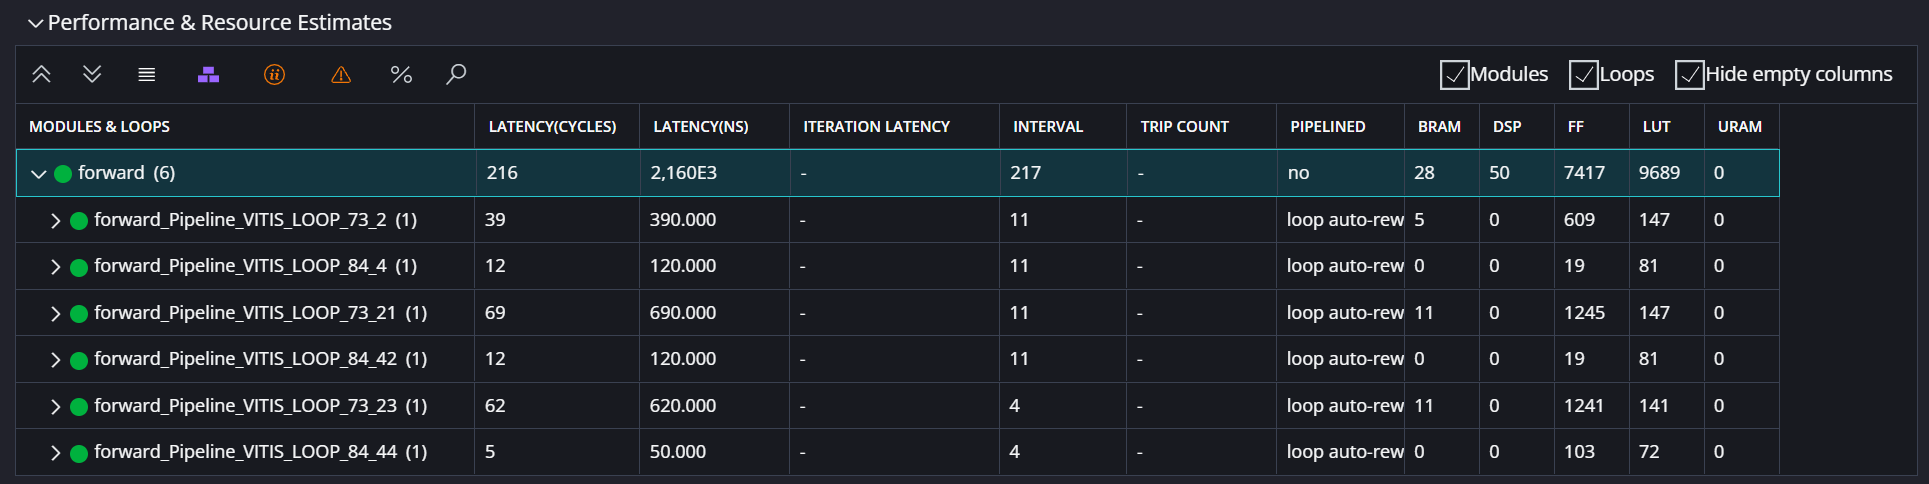
\includegraphics[width=1\textwidth]{./assets/MLP/c-synthesis-performanceandresourceestimaes.png}
    \caption{Perfomance and Resource Estimates in the C-Synthesis Report}
    \label{fig:convnet-c-synthesis-performance-resources-mlp}
\end{figure}


From the above image, we observe that the \texttt{forward} module exhibits an overall estimated latency of 216 cycles, corresponding to an execution time of 2,160 ns under the target clock frequency of 100 MHz (10 ns per cycle). The initiation interval (II) for the main module is reported as 217 cycles, which indicates that the design could benefit from further pipelining to optimize parallel execution and reduce the interval. Examining the resource utilization, the design employs:
\begin{itemize}
    \item \textbf{9,689 Look-Up Tables (LUTs)}, which corresponds to approximately 67.3\% of the total 14,400 LUTs available on the \texttt{xc7z007s-clg225-2}.
    \item \textbf{7,417 Flip-Flops (FFs)}, utilizing 25.7\% of the total 28,800 FFs available.
    \item \textbf{50 DSP slices}, accounting for 75.8\% of the total 66 available DSPs.
    \item \textbf{No BRAM (BlockRam) or URAM(UltraRam)}, which indicates that the design relies solely on external or internal registers for storage.
\end{itemize}

The internal loops of the \texttt{forward} pass module demonstrate varied latencies, with some loops optimized using \texttt{\#pragma HLS UNROLL} and \texttt{\#pragma HLS PIPELINE}. Latencies range from 5 ns to 690 ns, with the primary loop exhibiting the highest latency (690 ns). This latency suggests potential bottlenecks in data dependencies or resource contention, which could be addressed by restructuring loops or leveraging more efficient parallelization strategies.
\\\\We can also check from the report that, as expected, the hardware interface corresponds to the input and output of the forward pass function, and that the utilized pragma syntax is correct and corresponds to the one we used in the code.

\begin{figure}[H]
    \centering
    \begin{minipage}{0.49\textwidth}
        \centering
        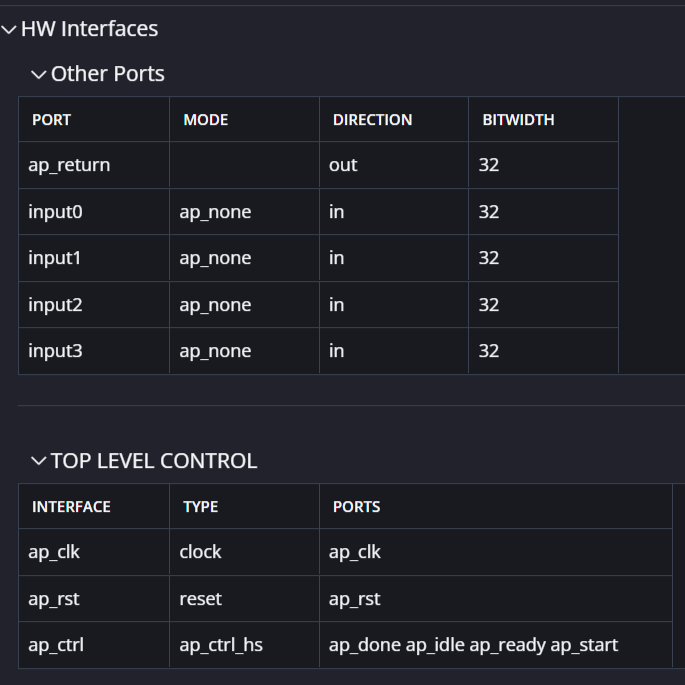
\includegraphics[width=1\textwidth]{./assets/MLP/c-synthesis-HWinterfaces.png}
        \caption{Hardware interfaces}
        \label{fig:c-synthesis-hw-interfaces}
    \end{minipage}
    \hfill
    \begin{minipage}{0.49\textwidth}
        \centering
        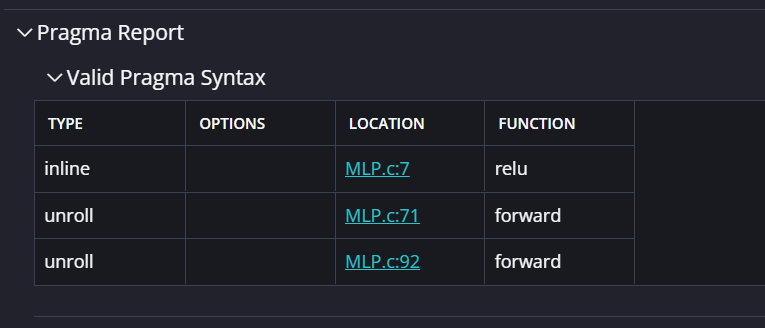
\includegraphics[width=1\textwidth]{./assets/MLP/c-synthesis-validpragmasyntax.png}
        \caption{Pragma syntax}
        \label{fig:c-synthesis-pragma-syntax}
    \end{minipage}
\end{figure}


\paragraph{C/RTL Simulation}

C-RTL cosimulation is a verification process that ensures the functional equivalence between the high-level C/C++ design and the synthesized Register-Transfer Level (RTL) code. This step is critical as it confirms that the behavior of the RTL implementation matches the original C/C++ description after synthesis. The benefits are multiple:

\begin{itemize}
    \item \textbf{Validation of Functional Correctness}: Verifies that the generated RTL implementation functions identically to the original high-level design for the same inputs.
    \item \textbf{Timing and Latency Estimates}: Provides insights into the actual timing behavior of the synthesized RTL.
    \item \textbf{Resource Utilization Check}: Highlights any discrepancies between resource usage reported during synthesis and actual utilization in hardware.
\end{itemize}

\subparagraph{How It Works}
\begin{enumerate}
    \item \textbf{Input Stimuli}: A testbench written in C/C++ is used to provide input data to both the high-level C/C++ design and the RTL design.
    \item \textbf{Output Comparison}: The outputs from the high-level simulation and the RTL simulation are compared.
    \item \textbf{Reports}: Any mismatches or timing violations are reported for debugging purposes.
\end{enumerate}


\begin{figure}[H]
    \centering
    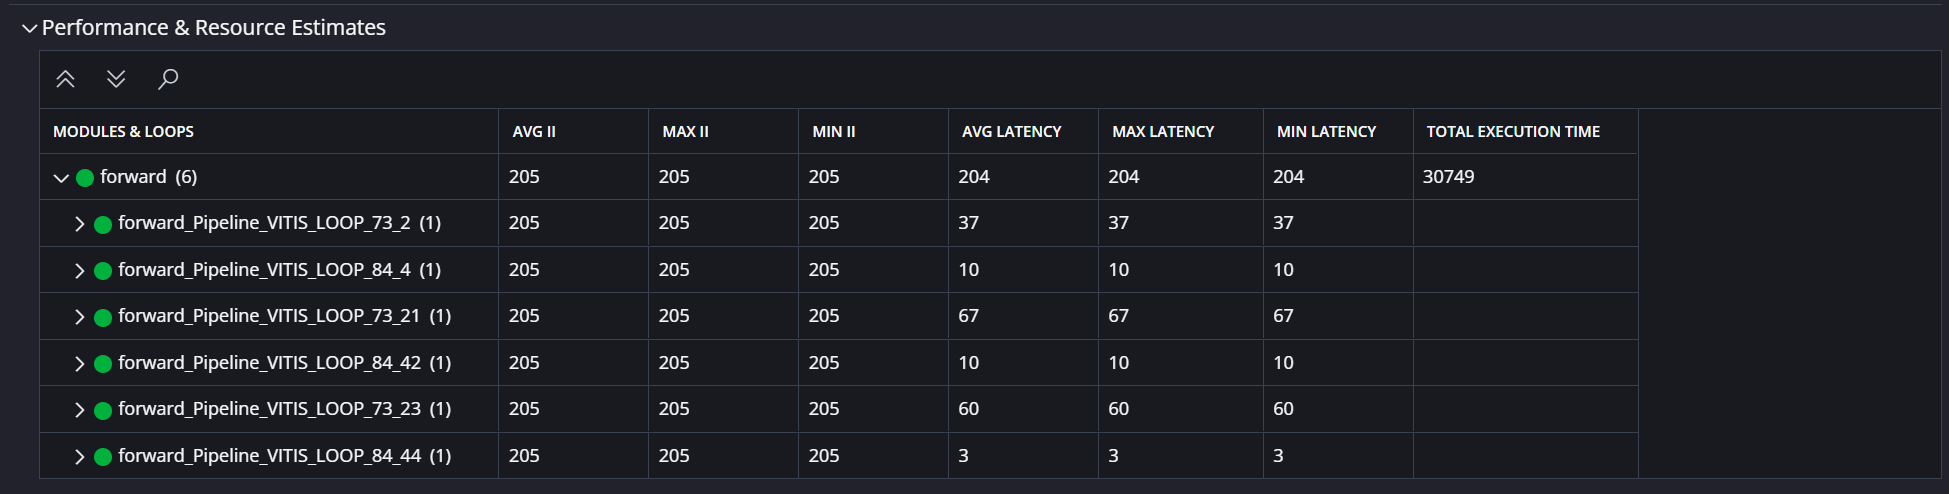
\includegraphics[width=1\textwidth]{./assets/MLP/c-rtl-cosimulation.png}
    \caption{C/RTL Cosimulation Report - Performance and resource estimates}
    \label{fig:C-RTL-cosimulation-mlp}
\end{figure}


From an analysis of the results from the C/RTL co-simulation and synthesis, we can highlights several key observations and metrics:

\begin{itemize}
    \item \textbf{Initiation Interval (II):} The initiation interval across all loops in the design remains constant at \textbf{205 cycles}. It indicates that certain dependencies or resource constraints may limit further reduction of the II.

    \item \textbf{Loop Latencies:} The latencies for individual loops vary significantly:
    \begin{itemize}
        \item The loop labeled \texttt{forward\_Pipeline\_VITIS\_LOOP\_73\_2} exhibits an average latency of \textbf{37 cycles}, which aligns with expectations for its complexity.
        \item Other loops, such as \texttt{forward\_Pipeline\_VITIS\_LOOP\_84\_44}, achieve minimal latencies of just \textbf{3 cycles}, indicating highly efficient implementation.
    \end{itemize}
    The overall latency of the forward pass main module is \textbf{204 cycles}, which matches the expected values from the high-level design.

    \item \textbf{Total Execution Time:} The total execution time for the forward pass is reported as 30,749 ns. This result reflects the aggregated runtime of all components and their interactions.

    \item \textbf{Pipeline Observations:} While the loops in the forward pass are pipelined, the relatively high initiation interval (205 cycles) suggests potential bottlenecks. These could stem from data dependencies or limited resource availability, particularly in critical paths of the design.

    \item \textbf{Resource Utilization:} 
    \begin{itemize}
        \item The design effectively utilizes available DSPs, LUTs, and Flip-Flops, as previously described.
        \item However, no usage of BRAM or URAM is reported. Leveraging these resources could reduce dependency on external memory and improve performance in memory-intensive operations.
    \end{itemize}
\end{itemize}

\paragraph{Observations and Suggestions}
The results confirm that the design is functional and performs as expected. However, several areas for improvement are identified:
\begin{enumerate}
    \item \textbf{Reducing II:} Efforts should be directed towards decreasing the initiation interval by addressing resource contention and loop dependencies. Techniques such as loop unrolling or splitting could be beneficial.
    \item \textbf{Memory Utilization:} Introducing BRAM or URAM for intermediate data storage can minimize external memory accesses and improve throughput.
    \item \textbf{Optimization of Critical Loops:} High-latency loops should be reviewed and restructured to enhance parallelism, potentially improving the overall execution time.
\end{enumerate}

By implementing these optimizations, the design could achieve higher efficiency and better alignment with the hardware capabilities of the target FPGA device.

\paragraph{Packaging}
Regarding the \textit{Package} section, there is  not much to be said, since the Vitis IDE doesn't provide a report for this stage. However, we can still infer that the packaging process was successful.

\paragraph{Implementation}

Here in this section we can mainly analyze the \textit{RTL synthesis} and the \textit{Place and Route} stages: the first provides a detailed report on the synthesis of the design into Register-Transfer Level (RTL) code, while the latter focuses on the physical implementation of the design on the FPGA.
Regarding the \textit{RTL synthesis}, the report provides insights into the resource utilization, timing constraints, and design hierarchy. The metrics include the number of Look-Up Tables (LUTs), Flip-Flops (FFs), and Digital Signal Processors (DSPs) used, as well as the critical path delay and maximum frequency. These metrics are crucial for assessing the design's efficiency and performance, guiding further optimization efforts.
\\\\ 

\paragraph{Fail Fast Analysis Overview:}

The Fail Fast analysis is a preliminary verification step designed to ensure that the design adheres to fundamental guidelines before proceeding to computationally intensive stages such as placement and routing. This stage evaluates key aspects of the design, including resource utilization and timing constraints, to identify potential bottlenecks early in the development process.

The following columns are analyzed:

\begin{itemize}
    \item \textbf{Criteria:} Key aspects of the design, such as LUT usage, FD (Flip-Flop Density), and DFP (Dynamic Floating-Point operations), are monitored to ensure they fall within acceptable thresholds.
    \item \textbf{Guideline:} Defines a reference threshold for each criterion to guide the design toward optimal FPGA resource usage and performance.
    \item \textbf{Actual:} Displays the measured values of each criterion after the analysis of the current design.
    \item \textbf{State:} Indicates the compliance status of each criterion, with possible values:
    \begin{itemize}
        \item \textbf{OK:} The criterion satisfies the guideline and requires no action.
        \item \textbf{WARNING:} The criterion approaches the threshold, suggesting caution.
        \item \textbf{FAIL:} The criterion exceeds the guideline, necessitating immediate attention.
    \end{itemize}
\end{itemize}

\paragraph{Criteria Evaluated:}
\begin{itemize}
    \item \textbf{LUT Usage:} Monitors the utilization of Look-Up Tables, ensuring that logic mapping remains within device capacity.
    \item \textbf{Flip-Flop Density:} Assesses the distribution of flip-flops to avoid routing congestion.
    \item \textbf{DSP Allocation:} Evaluates the usage of DSP slices for arithmetic operations, critical for neural network implementations.
    \item \textbf{Timing Constraints:} Verifies whether the design meets the required clock period and ensures no timing violations.
\end{itemize}

\subsubsection{RTL Synthesis and Fail Fast Analysis}

\begin{table}[H]
    \centering
    \makebox[\linewidth]{
    \begin{tabular}{|l|c|c|c|}
    \hline
    \textbf{Criteria} & \textbf{Guideline (\%)} & \textbf{Actual (\%)} & \textbf{Status} \\ \hline
    LUT               & 70                      & 30.82               & OK              \\ \hline
    FD                & 50                      & 18.51               & OK              \\ \hline
    LUTRAM+SRL        & 25                      & 1.73                & OK              \\ \hline
    MUXF7             & 15                      & 0.03                & OK              \\ \hline
    DSP               & 80                      & 75.76               & OK              \\ \hline
    RAMB/FIFO         & 80                      & 11.00               & OK              \\ \hline
    DSP+RAMB+URAM (Avg) & 70                    & 43.38               & OK              \\ \hline
    BUFGCE* + BUFGCTRL & 24                     & 0                   & OK              \\ \hline
    DONT\_TOUCH (cells/nets) & 0               & 0                   & OK              \\ \hline
    MARK\_DEBUG (nets) & 0                     & 0                   & OK              \\ \hline
    Control Sets      & 270                     & 86                  & OK              \\ \hline
    Average Fanout for modules $>$ 100k cells & 4 & 2.31            & OK              \\ \hline
    Max Average Fanout for modules $>$ 100k cells & 4 & 0            & OK              \\ \hline
    Non-FD high fanout nets $>$ 10k loads & 0    & 0                   & OK              \\ \hline
    TIMING-6 (No common primary clock between related clocks)          & 0                  & 0               & OK              \\ \hline
    TIMING-7 (No common node between related clocks)                   & 0                  & 0               & OK              \\ \hline
    TIMING-8 (No common period between related clocks)                 & 0                  & 0               & OK              \\ \hline
    TIMING-14 (LUT on the clock tree)                                  & 0                  & 0               & OK              \\ \hline
    TIMING-35 (No common node in paths with the same clock)            & 0                  & 0               & OK              \\ \hline
    Number of paths above max LUT budgeting (0.250ns)                 & 0                  & 0               & OK              \\ \hline
    Number of paths above max Net budgeting (0.177ns)                 & 0                  & 0               & OK              \\ \hline
    \end{tabular}
    }
    \caption{\centering Resource Utilization: RTL Synthesis Fail Fast}
    \label{tab:mlp-failfast-summary}
\end{table}

\begin{table}[H]
    \centering
    \begin{tabular}{|l|c|}
        \hline
        \textbf{Resource} & \textbf{Utilization} \\
        \hline
        SLICE & 0 \\
        LUT & 4,337 \\
        FF & 5,404 \\
        DSP & 50 \\
        BRAM & 11 \\
        URAM & 0 \\
        LATCH & 0 \\
        SRL & 104 \\
        CLB & 0 \\
        \hline
    \end{tabular}

    \vspace{5mm}

    \begin{tabular}{|l|c|}
        \hline
        \textbf{Timing Metric} & \textbf{Value} \\
        \hline
        Target Clock Period & 10.000 ns \\
        Post-Synthesis Clock Period & 6.872 ns \\
        Post-Implementation Clock Period & N/A \\
        \hline
    \end{tabular}

    \caption{Vivado RTL Synthesis Resource Summary and Timing}
\end{table}

\paragraph{Resource Utilization and Timing Analysis:}
The resource utilization for the RTL synthesis of the MLP forward pass implementation remains well within the acceptable limits, as shown in the provided tables. The LUT, FF, and DSP utilization values demonstrate efficient use of FPGA resources while maintaining a balanced design. The timing analysis confirms that the post-synthesis clock period of 6.872 ns is comfortably below the target clock period of 10.000 ns, ensuring the design's ability to meet performance constraints. However, the post-implementation clock period is not available, which indicates that further analysis during the place-and-route phase is necessary to verify final timing metrics.

\paragraph{Fail Fast Results Analysis:}
The fail fast analysis for the RTL synthesis phase indicates that all criteria have been met, with no violations reported. Resource utilization such as LUTs, FFs, and DSPs falls below the specified guidelines, ensuring that the design is both efficient and scalable. Additionally, there are no high fanout nets or other timing-related issues, confirming that the design is well-optimized at this stage. The results suggest that the design is ready for the subsequent place-and-route phase with no significant concerns, enabling seamless progression in the FPGA implementation process.




\subsubsection{Place \& Route and Fail Fast Analysis}

\begin{table}[H]
    \centering
    \makebox[\linewidth]{
    \begin{tabular}{|l|c|c|c|}
    \hline
    \textbf{Criteria} & \textbf{Guideline (\%)} & \textbf{Actual (\%)} & \textbf{Status} \\ \hline
    LUT               & 70                      & 25.96               & OK              \\ \hline
    FD                & 50                      & 18.63               & OK              \\ \hline
    LUTRAM+SRL        & 25                      & 1.73                & OK              \\ \hline
    MUXF7             & 15                      & 0.00                & OK              \\ \hline
    DSP               & 80                      & 75.76               & OK              \\ \hline
    RAMB/FIFO         & 80                      & 11.00               & OK              \\ \hline
    DSP+RAMB+URAM (Avg) & 70                    & 43.38               & OK              \\ \hline
    BUFGCE* + BUFGCTRL & 24                     & 0                   & OK              \\ \hline
    DONT\_TOUCH (cells/nets) & 0               & 0                   & OK              \\ \hline
    MARK\_DEBUG (nets) & 0                     & 0                   & OK              \\ \hline
    Control Sets      & 270                     & 78                  & OK              \\ \hline
    Average Fanout for modules $>$ 100k cells & 4 & 2.23            & OK              \\ \hline
    Max Average Fanout for modules $>$ 100k cells & 4 & 0            & OK              \\ \hline
    Non-FD high fanout nets $>$ 10k loads & 0    & 0                   & OK              \\ \hline
    TIMING-6 (No common primary clock between related clocks)          & 0                  & 0               & OK              \\ \hline
    TIMING-7 (No common node between related clocks)                   & 0                  & 0               & OK              \\ \hline
    TIMING-8 (No common period between related clocks)                 & 0                  & 0               & OK              \\ \hline
    TIMING-14 (LUT on the clock tree)                                  & 0                  & 0               & OK              \\ \hline
    TIMING-35 (No common node in paths with the same clock)            & 0                  & 0               & OK              \\ \hline
    Number of paths above max LUT budgeting (0.350ns)                 & 0                  & 0               & OK              \\ \hline
    Number of paths above max Net budgeting (0.177ns)                 & 0                  & 0               & OK              \\ \hline
    \end{tabular}
    }
    \caption{Resource Utilization: Place \& Route Fail Fast Summary}
    \label{tab:place-route-failfast-summary}
\end{table}

\vspace{5mm}

\begin{table}[H]
    \centering
    \begin{tabular}{|l|c|}
        \hline
        \textbf{Resource} & \textbf{Utilization} \\ \hline
        SLICE & 1,518 \\ \hline
        LUT & 3,738 \\ \hline
        FF & 5,364 \\ \hline
        DSP & 50 \\ \hline
        BRAM & 11 \\ \hline
        URAM & 0 \\ \hline
        LATCH & 0 \\ \hline
        SRL & 104 \\ \hline
        CLB & 0 \\ \hline
    \end{tabular}

    \vspace{5mm}

    \begin{tabular}{|l|c|}
        \hline
        \textbf{Timing Metric} & \textbf{Value} \\ \hline
        Target Clock Period & 10.000 ns \\ \hline
        Post-Synthesis Clock Period & 6.872 ns \\ \hline
        Post-Implementation Clock Period & 7.860 ns \\ \hline
    \end{tabular}
    \caption{Vivado Place \& Route Resource Summary and Timing}
    \label{tab:place-route-resource-timing}
\end{table}

\paragraph{Resource Utilization and Timing Analysis:}
The Place \& Route phase provides a detailed overview of the final resource usage and timing performance. The design consumes 3,738 LUTs, 5,364 FFs, 50 DSP blocks, 11 BRAMs, and 104 SRLs, while not utilizing any URAM, latches, or CLBs. The resource utilization demonstrates efficient use of the FPGA without exceeding critical limits, confirming the robustness of the implementation. 

For timing constraints, the target clock period is set to 10.000 ns, corresponding to a frequency of 100 MHz. During the synthesis stage, the achieved clock period was reported as 6.872 ns. Post-implementation, the clock period increased to 7.860 ns, accounting for additional routing delays and placement complexities. Despite this increase, the design still meets the required constraints, providing a sufficient margin for stable operation. The results confirm that the design is capable of operating within the specified timing requirements post-routing, reflecting an efficient and reliable implementation.

\paragraph{Fail Fast Results Analysis:}
The Fail Fast analysis for the Place \& Route phase reveals that all criteria are marked as \texttt{OK}, indicating full compliance with resource and timing guidelines. The resource utilization across LUTs, FFs, DSPs, and BRAMs is well-balanced, and the average fanout and control sets remain within acceptable ranges. The achieved clock period of 7.860 ns confirms timing compliance, demonstrating that routing and placement phases were successfully managed to maintain performance integrity.

Notably, the DSP utilization is at 75.8\%, suggesting an opportunity for optimization in future iterations, such as redistributing computational loads across LUTs or exploring alternative arithmetic implementations. The analysis further highlights the effective balance between resource utilization and timing constraints, ensuring a robust design suitable for FPGA acceleration.


\newpage


\section{Convolutional Neural Network (CNN)}
Convolutional Neural Networks (CNNs) are a class of deep learning models specifically designed to process grid-like data, such as images. Their ability to automatically learn spatial hierarchies of features makes them highly effective for image classification tasks. In this implementation, a simple yet efficient CNN is designed and trained to classify handwritten digits from the famuos MNIST dataset, with the aim of achieving high accuracy while remaining compatible with hardware synthesis constraints. So the ConvNet forward pass was implemented in a similar manner to the MLP, with the main difference being the convolution and pooling operations.


\subsection{Dataset}
The CNN was trained on the MNIST dataset, a widely used benchmark for handwritten digit classification tasks. The dataset consists of 70,000 grayscale images of digits (0,1,2,3,4,5,6,7,8,9), each with a resolution of $28 \times 28$ pixels. The dataset was split into two subsets, with 70\% used as the training set and 30\% as the validation set, resulting in the following distribution:

\begin{itemize}
    \item Training set: 42,000 samples.
    \item Validation set: 18,000 samples.
    \item Test set: 10,000 samples for evaluating the model's performance.
\end{itemize}

The dataset was preprocessed using normalization to scale pixel values to the range $[-1, 1]$, this normalization centers the pixel values around 0 and scales them to have a standard deviation of 1, which can often help with model training and convergence.


\subsection{PyTorch Model}

\subsubsection{Model Architecture}
The ConvNet is designed to be as simple as possible. The structure includes the following layers:
\begin{itemize}
    \item \textbf{Convolutional Layer:} A single convolutional layer with 3 filters, each of size $3 \times 3$, stride $1$, and padding $1$. This layer increases feature representation by extracting local patterns from the input images.
    \item \textbf{ReLU Activation:} Applied after the convolutional layer to introduce non-linearity into the model.
    \item \textbf{Pooling Layer:} A max-pooling layer with a kernel size of $2 \times 2$ and a stride of $2$, reducing the spatial dimensions of the feature map by half.
    \item \textbf{Fully Connected Layer:} It takes as input the flattened feature map from the convolutional and pooling layers. As output 10 neurons representing the 10 digit classes (0–9). This layer does not apply an activation function, it will be simply followed by \texttt{\textit{max(1)}} to obtain the predicted class.
\end{itemize}

The total number of parameters in this configuration is \textbf{5880}, which is relatively low compared to more complex CNN architectures. The forward pass through the network is done as follows:
\begin{enumerate}
    \item Apply the convolutional layer to the input image, followed by the ReLU activation function.
    \item Perform max-pooling on the resulting feature map to reduce spatial dimensions.
    \item Flatten the feature map into a one-dimensional vector.
    \item Pass the flattened vector through the fully connected layer to produce class probabilities.
\end{enumerate}

The simplicity of this architecture ensures compatibility with hardware synthesis while maintaining high accuracy for digit classification tasks.\\

The model was defined as follows, using the \textit{PyTorch} library:

\begin{lstlisting}[language=Python]
# Define the CNN model
class ConvNet(nn.Module):
    def __init__(self):
        super(ConvNet, self).__init__()
        # Input: x = [1, 28, 28]
        self.conv1 = nn.Conv2d(1, 3, kernel_size=3, stride=1, padding=1)  
        # Convolutional Layer: Output: x = [3, 28, 28]
        # Formula: (W - F + 2P) / S + 1
        self.pool = nn.MaxPool2d(kernel_size=2, stride=2)  
        # Pooling Layer: Output: x = [3, 14, 14]
        # Formula: (W - F) / S + 1
        self.fc1 = nn.Linear(3 * 14 * 14, 10)  
        # Fully Connected Layer: Flatten the output to match 10 classes

    def forward(self, x):
        x = torch.relu(self.conv1(x))  # Apply ReLU after convolution
        x = self.pool(x)              # Apply max pooling
        x = x.view(x.size(0), -1)     # Flatten the tensor
        x = self.fc1(x)               # Fully connected layer
        return x
\end{lstlisting}


\subsubsection{Model Training}
The training process for the Convolutional Neural Network (CNN) was performed using the \textit{PyTorch} library. The objective was to minimize the cross-entropy loss, a suitable loss function for multi-class classification problems. The training configuration was as follows:
\begin{itemize}
    \item \textbf{Loss Function:} CrossEntropyLoss.
    \item \textbf{Optimizer:} Adam optimizer with a learning rate of 0.001.
    \item \textbf{Batch Size:} 64.
    \item \textbf{Epochs:} 100.
\end{itemize}

\begin{lstlisting}[language=Python]
# initialize network, loss function and optimizer
model = ConvNet().to(device)
criterion = nn.CrossEntropyLoss()
optimizer = optim.Adam(model.parameters(), lr=learning_rate)
\end{lstlisting}

After each epoch, the model was evaluated on the validation set to monitor the training progress and prevent overfitting. The training and validation results at selected epochs are shown in the table below:

\begin{table}[htbp]
    \centering
    \label{tab:training-results}
    \renewcommand{\arraystretch}{1.2} % Increase row spacing
    \begin{tabular}{|c|c|c|c|c|}
    \hline
    \textbf{Epoch} & \textbf{Train Loss} & \textbf{Train Accuracy (\%)} & \textbf{Val Loss} & \textbf{Val Accuracy (\%)} \\ \hline
    10             & 0.1194             & 96.49                        & 0.1360            & 96.03                       \\ \hline
    20             & 0.0907             & 97.30                        & 0.1232            & 96.38                       \\ \hline
    30             & 0.0735             & 97.74                        & 0.1130            & 96.77                       \\ \hline
    40             & 0.0636             & 98.03                        & 0.1122            & 96.79                       \\ \hline
    50             & 0.0571             & 98.27                        & 0.1147            & 96.75                       \\ \hline
    60             & 0.0521             & 98.34                        & 0.1147            & 96.88                       \\ \hline
    70             & 0.0491             & 98.39                        & 0.1259            & 96.73                       \\ \hline
    80             & 0.0459             & 98.53                        & 0.1285            & 96.69                       \\ \hline
    90             & 0.0439             & 98.55                        & 0.1342            & 96.61                       \\ \hline
    100            & 0.0411             & 98.71                        & 0.1325            & 96.76                       \\ \hline
    \end{tabular}
    \caption{Training and Validation Results at Selected Epochs}
\end{table}
    

The final test performance was as follows:
\begin{itemize}
    \item \textbf{Test Loss:} 0.1260
    \item \textbf{Test Accuracy:} 97.06\%
\end{itemize}

Which can be considered good results, showing that the model was able to generalize well to unseen data even with only a "few" parameters and EPOCHs of training.\\

The following Python code snippet shows the main training loop:

\begin{lstlisting}[language=Python]
# Training loop
for epoch in range(NUM_EPOCHS):
    model.train()
    train_loss = 0.0
    train_correct = 0
    train_total = 0

    for images, labels in train_loader:
        images, labels = images.to(device), labels.to(device)

        optimizer.zero_grad()
        outputs = model(images)
        loss = criterion(outputs, labels)
        loss.backward()
        optimizer.step()

        train_loss += loss.item()
        _, predicted = outputs.max(1)
        train_total += labels.size(0)
        train_correct += predicted.eq(labels).sum().item()

    train_accuracy = 100. * train_correct / train_total

    # Validation phase
    model.eval()
    val_loss = 0.0
    val_correct = 0
    val_total = 0

    with torch.no_grad():  # Disable gradient calculations
        for images, labels in val_loader:
            images, labels = images.to(device), labels.to(device)

            outputs = model(images)
            loss = criterion(outputs, labels)

            val_loss += loss.item()
            _, predicted = outputs.max(1)
            val_total += labels.size(0)
            val_correct += predicted.eq(labels).sum().item()

    val_accuracy = 100. * val_correct / val_total

    if (epoch + 1) % 10 == 0:
        print(f"Epoch [{epoch + 1}/{NUM_EPOCHS}], "
              f"Train Loss: {train_loss / len(train_loader):.4f}, Train Acc: {train_accuracy:.2f}%, "
              f"Val Loss: {val_loss / len(val_loader):.4f}, Val Acc: {val_accuracy:.2f}%")
\end{lstlisting}



\subsubsection{Exporting Parameters}
To proceed with hardware implementation, the trained parameters (weights and biases) of the CNN model were exported to a structured format so that it could be easily loaded into the C implementation.
The following Python code was used to extract and store the parameters:

\begin{lstlisting}[language=Python]
with open('./convnet_weights.txt', 'w') as f:
    for name, weight in weights.items():
        f.write(f"// {name}, shape: {weight.shape}\n")
        
        if weight.ndim == 4:  # Convolutional weights: [out_channels, in_channels, kernel_height, kernel_width]
            for oc, w_slice in enumerate(weight):  # Iterate over output channels
                f.write(f"{{ // Output Channel {oc}\n")
                for row in w_slice:  # Iterate over rows (flattened kernels)
                    f.write("  {" + ", ".join(map(str, row.flatten())) + "},\n")
                f.write("},\n")
        
        elif weight.ndim == 2:  # Fully connected layer weights
            for row in weight:
                f.write("{" + ", ".join(map(str, row)) + "},\n")
        
        elif weight.ndim == 1:  # Biases or 1D weights
            f.write("{")
            f.write(", ".join(map(str, weight)) + "},\n")
    
\end{lstlisting}

This code snippet exports the weights and biases of the ConvNet model to the \texttt{convnet\_weights.txt} file. From it, the weights and biases for each layer can be simply copy-pasted inside the \texttt{ConvNet} structure in the C implementation. 

\subsection{C Implementation}
The implementation of the Convolutional Neural Network (CNN) model in C is divided into three main files:

\begin{itemize}
    \item \texttt{ConvNet.h}: This header file defines the data structures and constants used in the implementation, including the convolutional and fully connected layers, and the overall network structure.
    \item \texttt{ConvNet.c}: This file contains the implementation of the CNN's functionality, including the forward pass and activation functions, along with predefined weights and biases.
    \item \texttt{testbench.c}: This file serves as a testbench to verify the network's functionality. It includes functions for reading input data, executing the forward pass, and evaluating the model's output against the expected results.
\end{itemize}

The details of each file are described in the following subsections. The device used in this case was the \texttt{xczu15eg-ffvc900-3-e}, from the \textit{Zynq UltraScale+} family.

\begin{figure}[H]
    \centering
    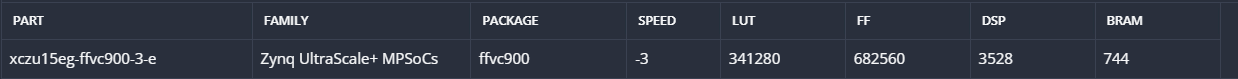
\includegraphics[width=1\textwidth]{./assets/ConvNet/device-used.png}
    \caption{Perfomance and Resource Estimates in the C-Synthesis Report}
    \label{fig:convent-device}
\end{figure}


\subsubsection{CNN Structure}
The Convolutional Neural Network (CNN) structure is implemented in C to match the architecture defined in the PyTorch model. Going into the details, the CNN consists of the following layers and operations:

\begin{itemize}
    \item \textbf{Convolutional Layer:} This layer performs the convolution operation by \textit{sliding} a set of filters (or \textbf{kernels}) over the input image to extract spatial features. The implementation uses nested loops to apply the filters, taking into account padding and stride.
    \item \textbf{ReLU Activation:} The Rectified Linear Unit (ReLU) activation function is applied after the convolutional operation to introduce non-linearity. The ReLU function replaces negative values in the feature map with zeros, its formulas was already provided in the MLP section.
    \item \textbf{Pooling Layer:} A max-pooling operation reduces the spatial dimensions of the feature map by selecting the maximum value within a kernel-sized region. This layer helps to downsample the feature map and make the model more robust to small spatial variations.
    \item \textbf{Fully Connected Layer:} The fully connected layer takes the flattened output from the pooling layer as input and maps it to the output classes. This is achieved by performing a linear transformation using the preloaded weights and biases.
\end{itemize}


\begin{figure}[H]
    \centering
    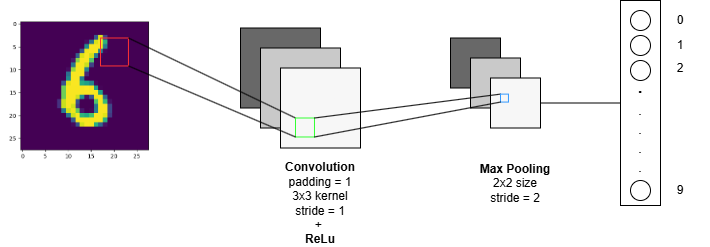
\includegraphics[width=1\textwidth]{./assets/ConvNet/convNet.png}
    \caption{Convolutional Neural Network Architecture}
    \label{fig:convolutional-neural-network}
\end{figure}


The CNN structure is defined in the header file \texttt{ConvNet.h}, which outlines the data structures and constants used for the network. Here the ConvNet structure:

\begin{lstlisting}[language=C]
// Structure to represent a convolutional layer
typedef struct {
    float weights[CONV1_OUTPUT_CHANNELS][INPUT_CHANNELS][3][3]; // Filters of the convolutional layer 
    float biases[CONV1_OUTPUT_CHANNELS]; // Biases for the filters
} ConvLayer;

// Structure to represent a fully connected layer
typedef struct {
    float weights[NUM_CLASSES][FC1_INPUT_SIZE]; // Weights of the fully connected layer
    float biases[NUM_CLASSES]; // Biases of the fully connected layer
} FullyConnectedLayer;

// General structure of the network
typedef struct {
    ConvLayer conv1; // First convolutional layer
    FullyConnectedLayer fc1; // Fully connected layer
} ConvNet;
\end{lstlisting}

As for the MLP implementation, all weights and biases in the CNN are hardcoded and directly integrated into the \texttt{ConvNet.c} file, where they can be found at the top.

\subsubsection{Forward Pass}
The forward pass function propagates an input image through the Convolutional Neural Network (CNN) to generate class probabilities as the output. It sequentially applies operations such as convolution, activation, pooling, and fully connected layers.
\\\\The following C code implements the forward pass:

\begin{lstlisting}[language=C]
int forward(float input[INPUT_HEIGHT][INPUT_WIDTH][INPUT_CHANNELS], float output[NUM_CLASSES]) {
    
    // Convolutional layer output buffer
    float conv_output[CONV1_OUTPUT_CHANNELS][INPUT_HEIGHT][INPUT_WIDTH];
    
    // Convolutional layer operation
    // Loop over output channels
    convolutional_layer: for (int oc = 0; oc < CONV1_OUTPUT_CHANNELS; oc++) {
        // Loop over input height
        for (int h = 0; h < INPUT_HEIGHT; h++) {        

            // Temporary buffer for input data (with padding)
            // Kernel size is 3x3, with a 3-row buffer
            float temp_input[3][INPUT_WIDTH+2][INPUT_CHANNELS]; 
            
            // Load the input data into the buffer with padding
            // Load 3 rows of input data
            for (int i = 0; i < 3; i++) { 
                // Adjust row index for kernel centering
                int curr_h = h + i - 1;  
                // Input width with padding
                for (int w = 0; w < INPUT_WIDTH + 2; w++) { 
                    // Loop over input channels
                    for (int c = 0; c < INPUT_CHANNELS; c++) {
                        // Apply zero-padding for boundary conditions
                        if (curr_h >= 0 && curr_h < INPUT_HEIGHT && w-1 >= 0 && w-1 < INPUT_WIDTH) {
                            temp_input[i][w][c] = input[curr_h][w-1][c];
                        } else {
                            temp_input[i][w][c] = 0.0f;
                        }
                    }
                }
            }
            
            // Perform convolution for the current row of the output
            for (int w = 0; w < INPUT_WIDTH; w++) {
                // Initialize with bias value
                float sum = convnet.conv1.biases[oc]; 
                
                // Convolve the kernel with the input buffer
                // Loop over input channels
                for (int ic = 0; ic < INPUT_CHANNELS; ic++) { 
                    // Kernel height
                    for (int kh = 0; kh < 3; kh++) {      
                        // Kernel width    
                        for (int kw = 0; kw < 3; kw++) {      
                            sum += temp_input[kh][w + kw][ic] * convnet.conv1.weights[oc][ic][kh][kw];
                        }
                    }
                }
                // Apply ReLU activation function
                conv_output[oc][h][w] = reLu(sum); 
            }
        }
    }

    // MaxPooling layer output buffer
    float pool_output[CONV1_OUTPUT_CHANNELS][INPUT_HEIGHT / POOL_SIZE][INPUT_WIDTH / POOL_SIZE];

    // MaxPooling operation
    // Loop over output channels
    for (int oc = 0; oc < CONV1_OUTPUT_CHANNELS; oc++) { 
        // Loop over pooled height
        for (int h = 0; h < INPUT_HEIGHT / POOL_SIZE; h++) { 
            // Loop over pooled width
            for (int w = 0; w < INPUT_WIDTH / POOL_SIZE; w++) { 
                // Initialize with a very small value
                float max_val = -1e9; 
                // Pooling window height
                for (int ph = 0; ph < POOL_SIZE; ph++) { 
                    // Pooling window width
                    for (int pw = 0; pw < POOL_SIZE; pw++) { 
                        // Calculate input height index
                        int ih = h * POOL_SIZE + ph; 
                        // Calculate input width index
                        int iw = w * POOL_SIZE + pw; 
                        // Ensure within bounds
                        if (ih < INPUT_HEIGHT && iw < INPUT_WIDTH) { 
                            // Find max value in window
                            if (conv_output[oc][ih][iw] > max_val) { 
                                max_val = conv_output[oc][ih][iw];
                            }
                        }
                    }
                }
                // Store max value in pooled output
                pool_output[oc][h][w] = max_val; 
            }
        }
    }

    // Fully connected layer input buffer
    float fc_input[FC1_INPUT_SIZE];
    #pragma HLS ARRAY_PARTITION variable=fc_input complete

    // Flatten pooling output into a 1D array
    // Index for flattened array
    int idx = 0; 
    // Loop over output channels
    flatten: for (int oc = 0; oc < CONV1_OUTPUT_CHANNELS; oc++) { 
        // Loop over pooled height
        for (int h = 0; h < INPUT_HEIGHT / POOL_SIZE; h++) { 
            // Loop over pooled width
            for (int w = 0; w < INPUT_WIDTH / POOL_SIZE; w++) { 
                fc_input[idx++] = pool_output[oc][h][w];
            }
        }
    }

    // Fully connected layer computation
    // Loop over output classes
    fully_connected_loop: for (int o = 0; o < NUM_CLASSES; o++) { 
        // Initialize with bias value
        float sum = convnet.fc1.biases[o]; 
        #pragma HLS PIPELINE II=1
        // Loop over flattened input
        for (int i = 0; i < FC1_INPUT_SIZE; i++) { 
            // Weighted sum of inputs
            sum += fc_input[i] * convnet.fc1.weights[o][i]; 
        }
        // Store the computed class score
        output[o] = sum; 
    }
    return 0; // Success
}
\end{lstlisting}

\subsubsection{Considerations on Pragmas and Forward-pass Code}

\begin{enumerate}
    \item \textbf{Array Partitioning (\texttt{\#pragma HLS ARRAY\_PARTITION})}:  
    The use of the \texttt{ARRAY\_PARTITION} pragma is important for improving parallelism, especially in operations that require concurrent access to multiple data elements. Partitioning arrays into independent variables, as in the case of the input array, convolution weights, and convolution output, allows the design to access different data in parallel without conflicts, improving efficiency. Completing the partition for each dimension of the array means that each element of the array is mapped to a separate hardware resource, enabling simultaneous access to the data. In the code, for example, applying \texttt{\#pragma HLS ARRAY\_PARTITION variable=fc\_input complete} within the forward function
    allows concurrent access to every element during the fully connected layer’s multiply-accumulate loops, thereby avoiding memory
    bottlenecks and improving overall throughput.

    \item \textbf{Pipeline (\texttt{\#pragma HLS PIPELINE})}:  
    The \texttt{PIPELINE} pragma is used to insert pipelining commands, which means operations can begin executing in parallel. The directive \texttt{II=1} reduces the initiation interval to 1 clock cycle, speeding up loop execution and reducing latency.

    This is particularly useful in loops where the operations are independent, such as in the convolution and max-pooling calculations. In the code of convolution loop, for instance, using \texttt{\#pragma HLS PIPELINE II=1} ensures that each new iteration can start
    processing in the next clock cycle, leading to significantly lower latency and higher throughput.


    \item \textbf{Efficiency of Convolution and Max-Pooling}\\
    Convolution and pooling are kept in separate, parallelizable loops, leveraging local buffers (such as the 3-row \texttt{temp\_input}) to handle padding and data retrieval. By loading only three rows of the input at a time, the design obtains precisely the rows needed by the $3 \times 3$ kernel at each step, improving memory usage and reducing overhead compared to storing extra unused rows. This targeted buffering approach minimizes the data transferred per output row, leading to better latency and throughput when combined with pipelining and partitioning directives.


    \item \textbf{Memory Efficiency and Buffer Management}\\
    Temporary buffers like the 3-row buffer for convolution and the intermediate arrays for outputs help manage partial computations and boundary conditions efficiently. However, it is important to size these buffers to match the actual kernel requirements, avoiding wasted storage and potential resource conflicts. By adopting a 3-row buffer specifically for a $3 \times 3$ kernel, the design loads only the necessary lines, reducing on-chip memory usage and preventing unnecessary data transfers.

\end{enumerate}

\subsubsection{Testbench}
The testbench reads input data from a file, processes it through the CNN using the \texttt{forward} function, and verifies the output against the expected label. This ensures that the implementation behaves as expected and aligns with the PyTorch model. The testbench performs the following tasks:

\begin{itemize}
    \item \textbf{Input Loading}: Reads the input image and its corresponding label from a text file (\texttt{input\_image.txt}), produced by the Jupyter Notebook. This has to be loaded inside the \textit{testbench} section of the Vitis IDE.
    \item \textbf{Forward Pass Execution}: Propagates the input through the CNN to compute class probabilities.
    \item \textbf{Result Validation}: Compares the predicted label with the true label and outputs the result.
\end{itemize}

The following code showcases the implementation of the testbench:

\begin{lstlisting}[language=C]
int main() {
    float input[INPUT_HEIGHT][INPUT_WIDTH][INPUT_CHANNELS];
    float output[NUM_CLASSES];
    int label;

    read_input_image(INPUT_FILE_PATH, input, &label);

    int results = forward(input, output);

    if (results != 0) {
        printf("Error during forward pass\n");
        return 1;
    }

    printf("Predicted output:\n");
    for (int i = 0; i < NUM_CLASSES; i++) {
        printf("Class %d: %f\n", i, output[i]);
    }

    float max_prob = output[0];
    int predicted_label = 0;

    for (int i = 1; i < NUM_CLASSES; i++) {
        if (output[i] > max_prob) {
            max_prob = output[i];
            predicted_label = i;
        }
    }
    printf("Predicted label: %d\n", predicted_label);
    printf("True label: %d\n", label);

    return 0;
}
\end{lstlisting}

Apart from the \texttt{read\_input\_image} (not reported here for brevity) we can see that the code follows the workflow explained above: reads an input image, passes it to the forward function, and then compares the predicted label with the true label.

\newpage
\subsection{Results}

\paragraph{Target Device}
The implementation of the Convolutional Neural Network forward pass on the FPGA was carried out on the Zynq UltraScale+ MPSoCs platform. The target device selected for this design was \texttt{xczu15eg-ffvc900-3-e}, which is part of the Zynq UltraScale+ family. The package used is \texttt{ffvc900}, with a speed grade of \texttt{-3}, this indicates that the target FPGA device is optimized for high performance, offering the fastest timing characteristics within its family. This makes it suitable for designs requiring high clock frequencies and low-latency operations, such as the convolutional neural network implementation.\\

The device offers the following key resources:
\begin{itemize}
    \item \textbf{LUTs:} 341,280
    \item \textbf{Flip-Flops (FFs):} 682,560
    \item \textbf{DSP slices:} 3,528
    \item \textbf{Block RAMs (BRAMs):} 744
\end{itemize}

This device was chosen for its high resource availability and support for efficient hardware acceleration, making it suitable for the implementation and optimization of the ConvNet design.


\subsubsection{Performance Metrics}
Let's dive into the results obtained inside the Vitis IDE for the simple convolutional neural network. 


\paragraph{C-Simulation}
As before, the first step is to run the C simulation to verify the correctness of the implementation. Here we could observe mainly the validity of the code: in the following image we report the output of the model with PyTorch and testbench one, showing the predicted label and the true label.

\begin{figure}[H]
    \centering
    \begin{minipage}{0.49\textwidth}
        \centering
        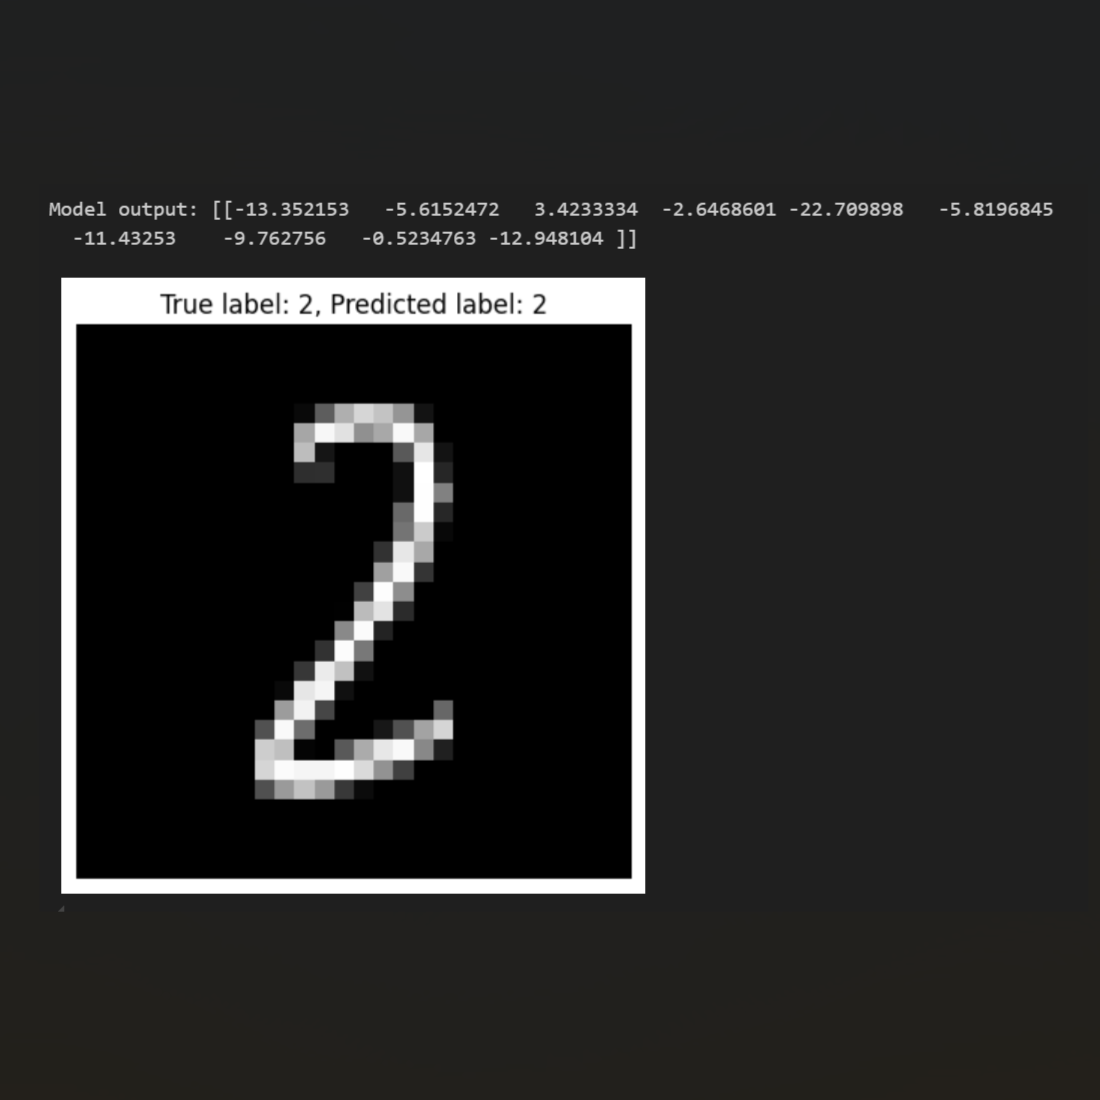
\includegraphics[width=1\textwidth]{assets/ConvNet/torch-prediction.png}
        \caption{PyTorch Model Prediction}
        \label{fig:convnet-torch-prediction}
    \end{minipage}
    \hfill
    \begin{minipage}{0.49\textwidth}
        \centering
        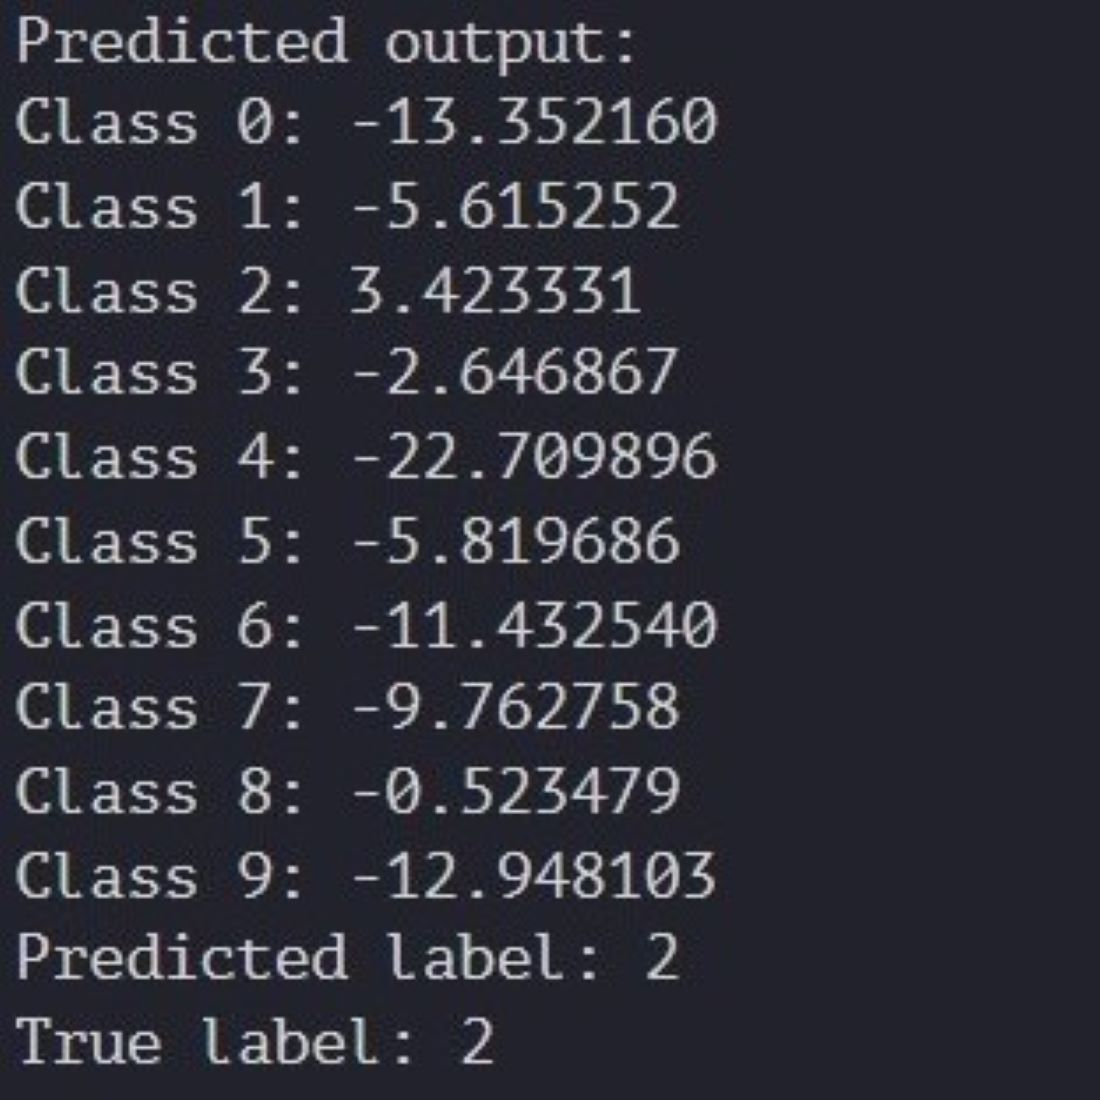
\includegraphics[width=1\textwidth]{assets/ConvNet/vitis-model-prediction.jpg}
        \caption{Prediction inside Vitis IDE}
        \label{fig:convnet-vitis-prediction}
    \end{minipage}
\end{figure}

As we can see, results are equal to the third decimal digit, which is a good sign that the C implementation is working as expected. As before, in the \textit{Code Analyer} section of the Vitis IDE, the message \texttt{A cyclic dependence prevents further acceleration of this process. This generally requires some algorithmic changes to improve}. As said for the MLP, this message is not a problem, but it's just a warning that the code could be optimized further.

\paragraph{C-Synthesis}
As for the MLP, we report the \textit{Estimated Quality of results} table:

\begin{table}[H]
    \centering
    \begin{tabular}{|c|c|c|}
        \hline
        \textbf{TARGET} & \textbf{ESTIMATED} & \textbf{UNCERTAINTY} \\
        \hline
        10.00 ns & 7.103 ns & 2.70 ns \\
        \hline
    \end{tabular}
    \caption{\centering Estimated Quality of Results for ConvNet Forward Pass}
    \label{tab:convnet-quality}
\end{table}

The estimated clock period is 7.103 ns, which is below the target of 10.00 ns, and this indicates that the design meets the timing constraints. The uncertainty of 2.70 ns represents the margin of error in the estimation, providing a range within which the actual performance may vary.

\begin{figure}[H]
    \centering
    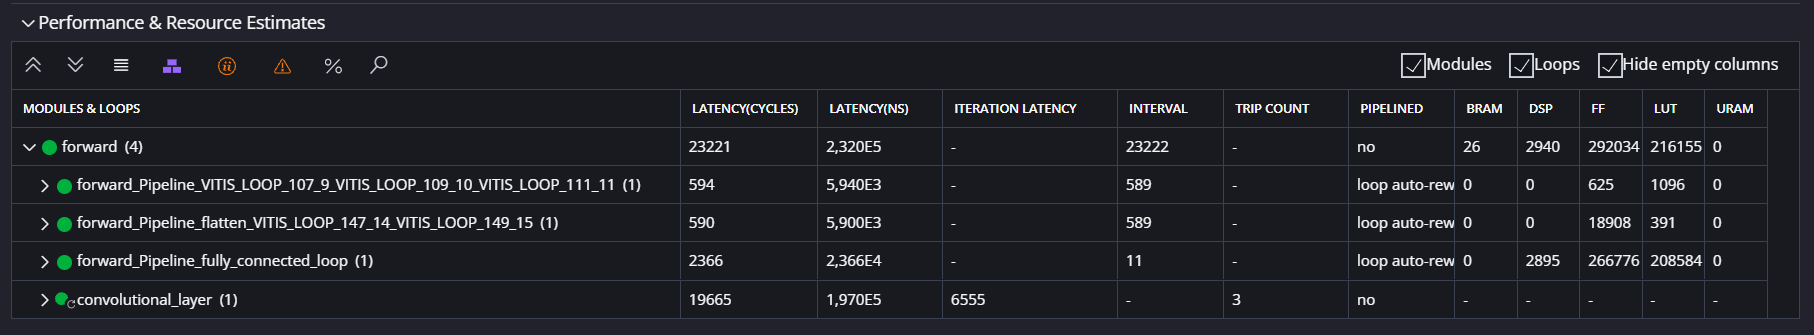
\includegraphics[width=1\textwidth]{./assets/ConvNet/c-synthesis-performanceandresourceestimates.png}
    \caption{Perfomance and Resource Estimates in the C-Synthesis Report}
    \label{fig:convnet-c-synthesis-performance-resources}
\end{figure}

From the above image, we observe that the \texttt{forward} module exhibits an overall estimated latency of \textbf{18,181 cycles}, corresponding to an execution time of approximately \textbf{182,010 ns} under the target clock frequency of 100 MHz (10 ns per cycle).

The \textbf{initiation interval (II)} for the \texttt{forward\_Pipeline\_fully\_connected\_loop} is reported as \textbf{11 cycles}, indicating a moderate level of pipelining. This implies that the loop can start a new iteration every 11 cycles. The \texttt{fully connected layer} within this module shows a latency of \textbf{2,366 cycles}, with the usage of 2,895 DSPs, 266,776 flip-flops (FFs), and 208,584 lookup tables (LUTs).

Similarly, the \texttt{convolutional layer} demonstrates a latency of \textbf{14,625 cycles}, with an iteration latency of 4,875 cycles and a trip count of 3. This layer makes significant use of BRAMs (26) and DSPs (2,940), as well as 292,026 FFs and 216,165 LUTs, highlighting the resource-intensive nature of this computation.
\\\\As we did for the MLP, let's also check from the report that the hardware interface corresponds to the input and output of the forward pass function, and that the utilized pragma syntax is correct.

\begin{figure}[H]
    \centering
    \begin{minipage}{0.49\textwidth}
        \centering
        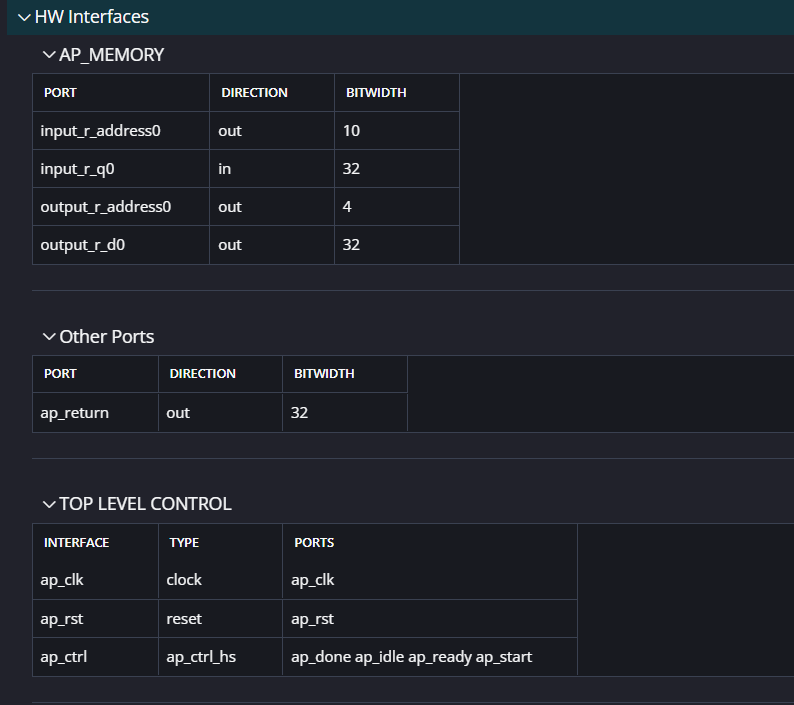
\includegraphics[width=1\textwidth]{./assets/ConvNet/c-synthesis-HWinterfaces.png}
        \caption{Hardware interfaces}
        \label{fig:convnet-c-synthesis-hw-interfaces}
    \end{minipage}
    \hfill
    \begin{minipage}{0.49\textwidth}
        \centering
        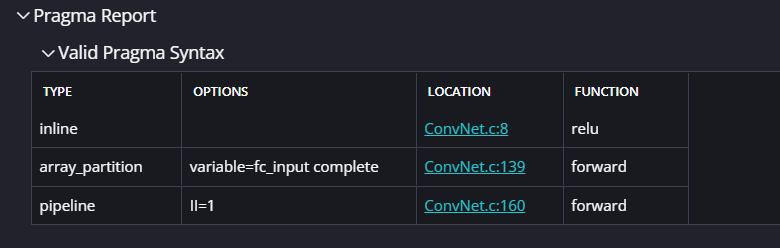
\includegraphics[width=1\textwidth]{./assets/ConvNet/c-synthesis-validpragmasyntax.png}
        \caption{Valid Pragma Softwareyntax}
        \label{fig:convnet-c-synthesis-pragma-syntax}
    \end{minipage}
\end{figure}


\paragraph{C/RTL Simulation}
The C/RTL simulation was performed to evaluate the performance and resource usage of the ConvNet design implemented for FPGA acceleration. This analysis focuses on key metrics, such as initiation interval (II), latency, and total execution time, to optimize the design's efficiency while maintaining correctness.

\begin{figure}[H]
    \centering
    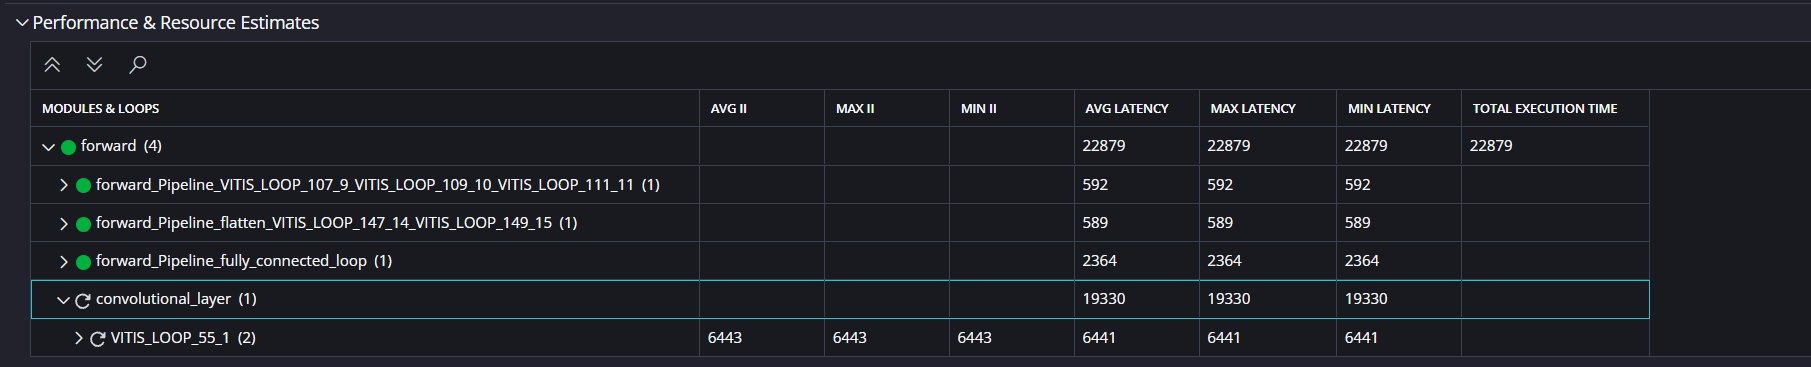
\includegraphics[width=1\textwidth]{./assets/ConvNet/c-rtl-cosimulation.png}
    \caption{C/RTL Cosimulation Report - Performance and resource estimates}
    \label{fig:C-RTL-cosimulation-convnet}
\end{figure}

The image above summarizes the breakdown of the simulation's key loops and modules. Each hierarchical level of the design is analyzed for critical factors affecting the throughput and latency:

\begin{itemize}
    \item The \texttt{forward} function is the top-level module, with a latency of \textbf{17,839 clock cycles}. This reflects the efficient design of the top-level module.
    \item Submodules within the \texttt{forward} function, such as \texttt{Pipeline\_flatten} and \texttt{Pipeline\_fully\_connected\_loop}, achieve low latency values (\textbf{592 cycles} and \textbf{2,364 cycles}, respectively) due to effective loop unrolling and partitioning strategies.
    \item The \texttt{convolutional\_layer} function exhibits a latency of \textbf{14,290 cycles}, showcasing its role as the most computationally intensive module in the hierarchy. This highlights the successful application of optimization techniques, such as array partitioning, ensuring maximum utilization of processing resources.
    \item The \texttt{VITIS\_LOOP\_55\_1} loop, part of the \texttt{convolutional\_layer}, demonstrates a significant latency of \textbf{4,763 cycles}, as it handles the critical computations of the kernel convolution. This indicates room for further optimization in kernel execution.
\end{itemize}


\paragraph{Packaging}
Regarding the Packaging section, there is not much to report, as the Vitis IDE does not generate a detailed report for this stage. However, it can be inferred that the packaging process was completed successfully, ensuring that the ConvNet design is ready for integration into larger FPGA-based systems.

\paragraph{Implementation}
In this section, we analyze the RTL Synthesis and the Place and Route stages of the ConvNet design implementation. These steps generate reports providing insights into the resource utilization, timing performance, and critical paths of the design, enabling further optimization and refinement.

During the implementation phase of the ConvNet design for FPGA acceleration, two important reports were generated:

\begin{itemize}
    \item \textbf{Vivado RTL Synthesis Report} (\texttt{hls\_impl\_syn.rpt})
    \item \textbf{Vivado Place \& Route Report} (\texttt{hls\_impl\_pnr.rpt})
\end{itemize}

These reports correspond to two critical steps in the FPGA design process: 

\subsubsection{RTL Synthesis and Fail Fast Analysis}
The synthesis step translates the high-level design into a register-transfer level (RTL) description. This involves:
\begin{itemize}
    \item Generating the hardware description in Verilog or VHDL.
    \item Estimating the resource utilization (LUTs, FFs, DSPs, BRAMs, etc.).
    \item Providing an initial assessment of the timing performance against the target clock period.
\end{itemize}

The results of the synthesis step are summarized in the tables below:

\begin{table}[H]
    \makebox[\linewidth]{
    \begin{tabular}{|l|c|c|c|}
    \hline
    \textbf{Criteria}                                                  & \textbf{Guideline} & \textbf{Actual (\%)} & \textbf{Status} \\ \hline
    LUT                                                               & 70\%               & 52.71\%              & OK              \\ \hline
    FD                                                                & 50\%               & 36.51\%              & OK              \\ \hline
    LUTRAM+SRL                                                        & 25\%               & 1.95\%               & OK              \\ \hline
    CARRY8                                                            & 25\%               & 16.69\%              & OK              \\ \hline
    MUXF7                                                             & 15\%               & 0.00\%               & OK              \\ \hline
    LUT Combining                                                     & 20\%               & 27.81\%              & REVIEW          \\ \hline
    DSP                                                               & 80\%               & 83.33\%              & REVIEW          \\ \hline
    RAMB/FIFO                                                         & 80\%               & 1.75\%               & OK              \\ \hline
    URAM                                                              & 80\%               & 0.00\%               & OK              \\ \hline
    DSP+RAMB+URAM (Avg)                                               & 70\%               & 42.54\%              & OK              \\ \hline
    BUFGCE* + BUFGCTRL                                                & 24                 & 0                    & OK              \\ \hline
    DONT\_TOUCH (cells/nets)                                          & 0                  & 0                    & OK              \\ \hline
    MARK\_DEBUG (nets)                                                & 0                  & 0                    & OK              \\ \hline
    Control Sets                                                      & 6399               & 3124                 & OK              \\ \hline
    Average Fanout for modules \textgreater 100k cells               & 4                  & 1.19                 & OK              \\ \hline
    Max Average Fanout for modules \textgreater 100k cells           & 4                  & 1.19                 & OK              \\ \hline
    Non-FD high fanout nets \textgreater 10k loads                   & 0                  & 0                    & OK              \\ \hline
    TIMING-6 (No common primary clock between related clocks)         & 0                  & 0                    & OK              \\ \hline
    TIMING-7 (No common node between related clocks)                  & 0                  & 0                    & OK              \\ \hline
    TIMING-8 (No common period between related clocks)                & 0                  & 0                    & OK              \\ \hline
    TIMING-14 (LUT on the clock tree)                                 & 0                  & 0                    & OK              \\ \hline
    TIMING-35 (No common node in paths with the same clock)           & 0                  & 0                    & OK              \\ \hline
    Number of paths above max LUT budgeting (0.250ns)                 & 0                  & 0                    & OK              \\ \hline
    Number of paths above max Net budgeting (0.177ns)                 & 0                  & 0                    & OK              \\ \hline
    \end{tabular}
    }
    \caption{Resource Utilization: RTL Synthesis Fail Fast}
\end{table}

    

\begin{table}[H]
    \centering
    \label{tab:rtl-synthesis-results}
    \begin{tabular}{|l|c|}
        \hline
        \textbf{Resource} & \textbf{Utilization} \\
        \hline
        LUT & 179,894 \\
        FF & 249,181 \\
        DSP & 2,940 \\
        BRAM & 26 \\
        URAM & 0 \\
        SRL & 3,306 \\
        \hline
    \end{tabular}

    \vspace{5mm}

    \begin{tabular}{|l|c|}
        \hline
        \textbf{Timing Metric} & \textbf{Value} \\
        \hline
        Target Clock Period & 10.000 ns \\
        Post-Synthesis Clock Period & 3.232 ns \\
        \hline
    \end{tabular}

    \caption{Vivado RTL Synthesis Resource Summary and Timing}
\end{table}

The synthesis results indicate that the design fits comfortably within the available resources of the target FPGA, but with the necessary attention on resources with REVIEW status, commented below.  The achieved clock period (3.232 ns) is well below the target period (10.000 ns), ensuring sufficient timing slack at this stage.

\paragraph{Fail Fast Results Analysis:}
The REVIEW status in the RTL Synthesis report indicates that specific resource usage metrics, such as DSP utilization (83.33\%) and LUT Combining (27.81\%), exceed their recommended thresholds (80\% and 20\%, respectively). While these values do not cause a failure, they suggest potential bottlenecks or inefficiencies that could impact overall design performance, in particular the DSP utilization is relatively high which might require attention during optimization.
\begin{itemize}
    \item \textbf{DSP Utilization}: DSP resources are slightly over the recommended guideline. While acceptable for synthesis, it may limit future scalability or integration with additional components.
    \item \textbf{LUT Combining}: The value exceeding the guideline indicates potential inefficiencies in logic mapping. We should consider that it is less critical than DSP utilization.
\end{itemize}

So, to determine whether these values are acceptable, we should consider the subsequent Place \& Route (PnR) Report, which provides post-implementation resource usage and timing analysis. If the PnR report will confirm that timing constraints are met and no routing congestion occurs, the design can be considered acceptable despite the REVIEW statuses in the RTL synthesis phase.

\subsubsection{Place \& Route and Fail Fast Analysis}
The place-and-route step maps the synthesized RTL onto the physical resources of the FPGA. This step provides:
\begin{itemize}
    \item The final resource utilization after physical implementation.
    \item The timing analysis considering routing delays.
    \item A pass/fail evaluation of key design metrics.
\end{itemize}

The results of the place-and-route step are summarized in the tables below:

\begin{table}[H]
    \makebox[\linewidth]{
    \begin{tabular}{|l|c|c|c|}
    \hline
    \textbf{Criteria}                                                  & \textbf{Guideline} & \textbf{Actual (\%)} & \textbf{Status} \\ \hline
    LUT                                                               & 70\%               & 44.13\%              & OK              \\ \hline
    FD                                                                & 50\%               & 36.25\%              & OK              \\ \hline
    LUTRAM+SRL                                                        & 25\%               & 1.84\%               & OK              \\ \hline
    CARRY8                                                            & 25\%               & 16.69\%              & OK              \\ \hline
    MUXF7                                                             & 15\%               & 0.00\%               & OK              \\ \hline
    DSP                                                               & 80\%               & 83.33\%              & REVIEW          \\ \hline
    RAMB/FIFO                                                         & 80\%               & 1.75\%               & OK              \\ \hline
    URAM                                                              & 80\%               & 0.00\%               & OK              \\ \hline
    DSP+RAMB+URAM (Avg)                                               & 70\%               & 42.54\%              & OK              \\ \hline
    BUFGCE* + BUFGCTRL                                                & 24                 & 0                    & OK              \\ \hline
    DONT\_TOUCH (cells/nets)                                          & 0                  & 0                    & OK              \\ \hline
    MARK\_DEBUG (nets)                                                & 0                  & 0                    & OK              \\ \hline
    Control Sets                                                      & 6399               & 2546                 & OK              \\ \hline
    Average Fanout for modules \textgreater 100k cells               & 4                  & 0.99                 & OK              \\ \hline
    Max Average Fanout for modules \textgreater 100k cells           & 4                  & 0.99                 & OK              \\ \hline
    Non-FD high fanout nets \textgreater 10k loads                   & 0                  & 0                    & OK              \\ \hline
    TIMING-6 (No common primary clock between related clocks)         & 0                  & 0                    & OK              \\ \hline
    TIMING-7 (No common node between related clocks)                  & 0                  & 0                    & OK              \\ \hline
    TIMING-8 (No common period between related clocks)                & 0                  & 0                    & OK              \\ \hline
    TIMING-14 (LUT on the clock tree)                                 & 0                  & 0                    & OK              \\ \hline
    TIMING-35 (No common node in paths with the same clock)           & 0                  & 0                    & OK              \\ \hline
    Number of paths above max LUT budgeting (0.250ns)                 & 0                  & 0                    & OK              \\ \hline
    Number of paths above max Net budgeting (0.177ns)                 & 0                  & 0                    & OK              \\ \hline
    \end{tabular}
    }
    \caption{Resource Utilization: Place \& Route Fail Fast}
\end{table}

\begin{table}[H]
    \centering
    \label{tab:place-route-results}
    \begin{tabular}{|l|c|}
        \hline
        \textbf{Resource} & \textbf{Utilization} \\
        \hline
        LUT & 150,621 \\
        FF & 247,414 \\
        DSP & 2,940 \\
        BRAM & 26 \\
        URAM & 0 \\
        SRL & 3,242 \\
        \hline
    \end{tabular}

    \vspace{5mm}

    \begin{tabular}{|l|c|}
        \hline
        \textbf{Timing Metric} & \textbf{Value} \\
        \hline
        Target Clock Period & 10.000 ns \\
        Post-Route Clock Period & 9.354 ns \\
        \hline
    \end{tabular}
    \caption{Vivado Place \& Route Resource Summary and Timing}
\end{table}

The resource utilization remains within acceptable limits after place-and-route, with slight changes compared to the synthesis stage. \paragraph{Timing Analysis:} The timing was successfully met, with a post-route clock period of 9.354 ns, which is below the target clock period. This indicates that the design is capable of operating at the desired frequency after routing delays are considered: the previously reported Post-Synthesis Clock Period of 3.232 ns reflects the timing achievable after synthesis, where the design is represented at a higher level of abstraction without considering physical constraints like placement and routing. In contrast, at this point we obtain a clock period of 9.354 ns that accounts for the additional delays introduced by the placement and routing phases, including wire propagation delays and congestion. Despite these variations, both timing values comfortably meet the Target Clock Period of 10.000 ns, ensuring that the design operates reliably within the specified timing constraints.

\paragraph{Fail Fast Results Analysis:}
The implementation phase results confirm that the design fits within the available resources and meets timing requirements. We have to note that the high DSP utilization (83.33\%) across both stages suggests potential optimization opportunities. However, the design is functional and meets the performance criteria, indicating successful implementation for FPGA acceleration.

\newpage
\section*{Final Remarks}

The implementation and analysis provided in this document are supported by the source code and additional resources available in the GitHub repository. The repository contains the complete project files, including code, configuration scripts, and detailed documentation.

\noindent You can access the GitHub repository at the following link:

\begin{figure}[H]
    \centering
    
\includegraphics[width=0.2\textwidth]{assets/github-logo.png}
    \label{fig:github}
\end{figure}

\begin{center}
\textbf{\url{https://github.com/giuliocapecchi/Vitis-HLS}} 
\end{center}

\end{document}